% Options for packages loaded elsewhere
\PassOptionsToPackage{unicode}{hyperref}
\PassOptionsToPackage{hyphens}{url}
%
\documentclass[
]{book}
\usepackage{amsmath,amssymb}
\usepackage{lmodern}
\usepackage{iftex}
\ifPDFTeX
  \usepackage[T1]{fontenc}
  \usepackage[utf8]{inputenc}
  \usepackage{textcomp} % provide euro and other symbols
\else % if luatex or xetex
  \usepackage{unicode-math}
  \defaultfontfeatures{Scale=MatchLowercase}
  \defaultfontfeatures[\rmfamily]{Ligatures=TeX,Scale=1}
\fi
% Use upquote if available, for straight quotes in verbatim environments
\IfFileExists{upquote.sty}{\usepackage{upquote}}{}
\IfFileExists{microtype.sty}{% use microtype if available
  \usepackage[]{microtype}
  \UseMicrotypeSet[protrusion]{basicmath} % disable protrusion for tt fonts
}{}
\makeatletter
\@ifundefined{KOMAClassName}{% if non-KOMA class
  \IfFileExists{parskip.sty}{%
    \usepackage{parskip}
  }{% else
    \setlength{\parindent}{0pt}
    \setlength{\parskip}{6pt plus 2pt minus 1pt}}
}{% if KOMA class
  \KOMAoptions{parskip=half}}
\makeatother
\usepackage{xcolor}
\usepackage{color}
\usepackage{fancyvrb}
\newcommand{\VerbBar}{|}
\newcommand{\VERB}{\Verb[commandchars=\\\{\}]}
\DefineVerbatimEnvironment{Highlighting}{Verbatim}{commandchars=\\\{\}}
% Add ',fontsize=\small' for more characters per line
\usepackage{framed}
\definecolor{shadecolor}{RGB}{248,248,248}
\newenvironment{Shaded}{\begin{snugshade}}{\end{snugshade}}
\newcommand{\AlertTok}[1]{\textcolor[rgb]{0.94,0.16,0.16}{#1}}
\newcommand{\AnnotationTok}[1]{\textcolor[rgb]{0.56,0.35,0.01}{\textbf{\textit{#1}}}}
\newcommand{\AttributeTok}[1]{\textcolor[rgb]{0.77,0.63,0.00}{#1}}
\newcommand{\BaseNTok}[1]{\textcolor[rgb]{0.00,0.00,0.81}{#1}}
\newcommand{\BuiltInTok}[1]{#1}
\newcommand{\CharTok}[1]{\textcolor[rgb]{0.31,0.60,0.02}{#1}}
\newcommand{\CommentTok}[1]{\textcolor[rgb]{0.56,0.35,0.01}{\textit{#1}}}
\newcommand{\CommentVarTok}[1]{\textcolor[rgb]{0.56,0.35,0.01}{\textbf{\textit{#1}}}}
\newcommand{\ConstantTok}[1]{\textcolor[rgb]{0.00,0.00,0.00}{#1}}
\newcommand{\ControlFlowTok}[1]{\textcolor[rgb]{0.13,0.29,0.53}{\textbf{#1}}}
\newcommand{\DataTypeTok}[1]{\textcolor[rgb]{0.13,0.29,0.53}{#1}}
\newcommand{\DecValTok}[1]{\textcolor[rgb]{0.00,0.00,0.81}{#1}}
\newcommand{\DocumentationTok}[1]{\textcolor[rgb]{0.56,0.35,0.01}{\textbf{\textit{#1}}}}
\newcommand{\ErrorTok}[1]{\textcolor[rgb]{0.64,0.00,0.00}{\textbf{#1}}}
\newcommand{\ExtensionTok}[1]{#1}
\newcommand{\FloatTok}[1]{\textcolor[rgb]{0.00,0.00,0.81}{#1}}
\newcommand{\FunctionTok}[1]{\textcolor[rgb]{0.00,0.00,0.00}{#1}}
\newcommand{\ImportTok}[1]{#1}
\newcommand{\InformationTok}[1]{\textcolor[rgb]{0.56,0.35,0.01}{\textbf{\textit{#1}}}}
\newcommand{\KeywordTok}[1]{\textcolor[rgb]{0.13,0.29,0.53}{\textbf{#1}}}
\newcommand{\NormalTok}[1]{#1}
\newcommand{\OperatorTok}[1]{\textcolor[rgb]{0.81,0.36,0.00}{\textbf{#1}}}
\newcommand{\OtherTok}[1]{\textcolor[rgb]{0.56,0.35,0.01}{#1}}
\newcommand{\PreprocessorTok}[1]{\textcolor[rgb]{0.56,0.35,0.01}{\textit{#1}}}
\newcommand{\RegionMarkerTok}[1]{#1}
\newcommand{\SpecialCharTok}[1]{\textcolor[rgb]{0.00,0.00,0.00}{#1}}
\newcommand{\SpecialStringTok}[1]{\textcolor[rgb]{0.31,0.60,0.02}{#1}}
\newcommand{\StringTok}[1]{\textcolor[rgb]{0.31,0.60,0.02}{#1}}
\newcommand{\VariableTok}[1]{\textcolor[rgb]{0.00,0.00,0.00}{#1}}
\newcommand{\VerbatimStringTok}[1]{\textcolor[rgb]{0.31,0.60,0.02}{#1}}
\newcommand{\WarningTok}[1]{\textcolor[rgb]{0.56,0.35,0.01}{\textbf{\textit{#1}}}}
\usepackage{longtable,booktabs,array}
\usepackage{calc} % for calculating minipage widths
% Correct order of tables after \paragraph or \subparagraph
\usepackage{etoolbox}
\makeatletter
\patchcmd\longtable{\par}{\if@noskipsec\mbox{}\fi\par}{}{}
\makeatother
% Allow footnotes in longtable head/foot
\IfFileExists{footnotehyper.sty}{\usepackage{footnotehyper}}{\usepackage{footnote}}
\makesavenoteenv{longtable}
\usepackage{graphicx}
\makeatletter
\def\maxwidth{\ifdim\Gin@nat@width>\linewidth\linewidth\else\Gin@nat@width\fi}
\def\maxheight{\ifdim\Gin@nat@height>\textheight\textheight\else\Gin@nat@height\fi}
\makeatother
% Scale images if necessary, so that they will not overflow the page
% margins by default, and it is still possible to overwrite the defaults
% using explicit options in \includegraphics[width, height, ...]{}
\setkeys{Gin}{width=\maxwidth,height=\maxheight,keepaspectratio}
% Set default figure placement to htbp
\makeatletter
\def\fps@figure{htbp}
\makeatother
\setlength{\emergencystretch}{3em} % prevent overfull lines
\providecommand{\tightlist}{%
  \setlength{\itemsep}{0pt}\setlength{\parskip}{0pt}}
\setcounter{secnumdepth}{5}
\usepackage{booktabs}
\usepackage{amsthm}
\usepackage{amssymb}
\makeatletter
\def\thm@space@setup{%
  \thm@preskip=8pt plus 2pt minus 4pt
  \thm@postskip=\thm@preskip
}
\makeatother
\usepackage[spanish]{babel}
\usepackage[utf8]{inputenc}
\spanishdecimal{.}
%\renewcommand{\contentsname}{Contenido}
\ifLuaTeX
  \usepackage{selnolig}  % disable illegal ligatures
\fi
\usepackage[]{natbib}
\bibliographystyle{apalike}
\nocite{xie2015, casale2012, roberts2008, erre2017, somolinos2010}
\IfFileExists{bookmark.sty}{\usepackage{bookmark}}{\usepackage{hyperref}}
\IfFileExists{xurl.sty}{\usepackage{xurl}}{} % add URL line breaks if available
\urlstyle{same} % disable monospaced font for URLs
\hypersetup{
  pdftitle={Introducción a la Programación con SAS IML},
  pdfauthor={Mgs. Lic. Marcos Prunello},
  hidelinks,
  pdfcreator={LaTeX via pandoc}}

\title{Introducción a la Programación con SAS IML}
\usepackage{etoolbox}
\makeatletter
\providecommand{\subtitle}[1]{% add subtitle to \maketitle
  \apptocmd{\@title}{\par {\large #1 \par}}{}{}
}
\makeatother
\subtitle{Guía para las clases}
\author{Mgs. Lic. Marcos Prunello}
\date{Última edición: 14-09-2019}

\begin{document}
\maketitle

{
\setcounter{tocdepth}{1}
\tableofcontents
}
\hypertarget{bienvenidos-al-taller}{%
\chapter{Bienvenidos al Taller}\label{bienvenidos-al-taller}}

La presente es una breve guía que resume los conceptos más importantes a desarrollar en el Taller de Programación de la Licenciatura en Estadística en la Facultad de Ciencias Económicas y Estadística, Universidad Nacional de Rosario, para las cursadas de 2017 a 2019. La misma no está exenta de presentar errores o expresar ideas que puedan ser mejoradas.

\hypertarget{horario-y-lugar-de-cursado}{%
\section*{Horario y lugar de cursado}\label{horario-y-lugar-de-cursado}}
\addcontentsline{toc}{section}{Horario y lugar de cursado}

Lunes de 8:00 a 12:00 en el Laboratorio de Computación de la Escuela de Estadística.

\hypertarget{consultas}{%
\section*{Consultas}\label{consultas}}
\addcontentsline{toc}{section}{Consultas}

A través del Foro de Consultas en el Campus Virtual o al finalizar las clases.

\hypertarget{material-de-estudio}{%
\section*{Material de estudio}\label{material-de-estudio}}
\addcontentsline{toc}{section}{Material de estudio}

El material de estudio está compuesto por esta guía, prácticas y algunas presentaciones en diapositivas, que, junto con cualquier otro material que necesitemos, estarán disponibles en nuestro espacio en el Campus Virtual de la UNR.

Todo el material disponible (guía, diapositivas, prácticas, publicación online) fue creado utilizando el lenguaje de programación estadística \texttt{R} y las herramientas del entorno de desarrollo integrado \texttt{RStudio}.

\hypertarget{evaluaciuxf3n}{%
\section*{Evaluación}\label{evaluaciuxf3n}}
\addcontentsline{toc}{section}{Evaluación}

Tendremos tres Actividades Evaluativas (AE) cuyos detalles serán explicados oportunamente en el cuatrimestre. Las tres notas se promediarán para obtener una Nota Final con las siguientes ponderaciones: 20\% AE1, 40\% AE2 y 40\% AE3. Si la Nota Final es mayor o igual a ocho (8), se promueve la materia; si es es mayor o igual a seis (6) y menor a ocho (8), se alcanza la condición de regular; y si es menor a seis (6), el alumno es libre.

Habrá una única instancia opcional de recuperación al final del cuatrimestre de carácter integrador para aquellos que no alcanzaron la promoción, cuya nota no reemplaza a ninguna actividad evalulativa. Si la misma es mayor o igual a ocho (8) se alcanza la promoción y en caso contrario se conserva la condición ya obtenida.

\hypertarget{campus-virtual}{%
\section*{Campus virtual}\label{campus-virtual}}
\addcontentsline{toc}{section}{Campus virtual}

Además de alojar todo el material del curso, utilizaremos este espacio para la entrega de trabajos y para realizar consultas, que esperamos puedan ser debatidas y respondidas entre los mismos estudiantes.

\hypertarget{introducciuxf3n}{%
\chapter{Introducción}\label{introducciuxf3n}}

\hypertarget{una-breve-reseuxf1a-histuxf3rica-sobre-la-computaciuxf3n}{%
\section{Una breve reseña histórica sobre la computación}\label{una-breve-reseuxf1a-histuxf3rica-sobre-la-computaciuxf3n}}

La palabra \textbf{computación} proviene del latín \emph{computatio}, que deriva del verbo \emph{computare}, cuyo significado es ``enumerar cantidades''. Computación, en este sentido, designa la acción y efecto de computar, realizar una cuenta, un cálculo matemático. De allí que antiguamente computación fuese un término usado para referirse a los cálculos realizados por una persona con un instrumento expresamente utilizado para tal fin (como el ábaco, por ejemplo) o sin él. En este sentido, la computación ha estado presente desde tiempos ancestrales.

A través de la historia, la computación progresó de manera relativamente lenta. En 1623, el alemán Wilhelm Schickard inventó la primera calculadora mecánica, capaz de realizar cómputos aritméticos sencillos. Este, y otros modelos posteriores, eran puramente mecánicos, sin motores ni otras fuentes de energía. El operador ingresaba números ubicando ruedas de metal en posiciones particulares y al girarlas otras partes de la máquina se movían y mostraban el resultado.

\begin{figure}

{\centering 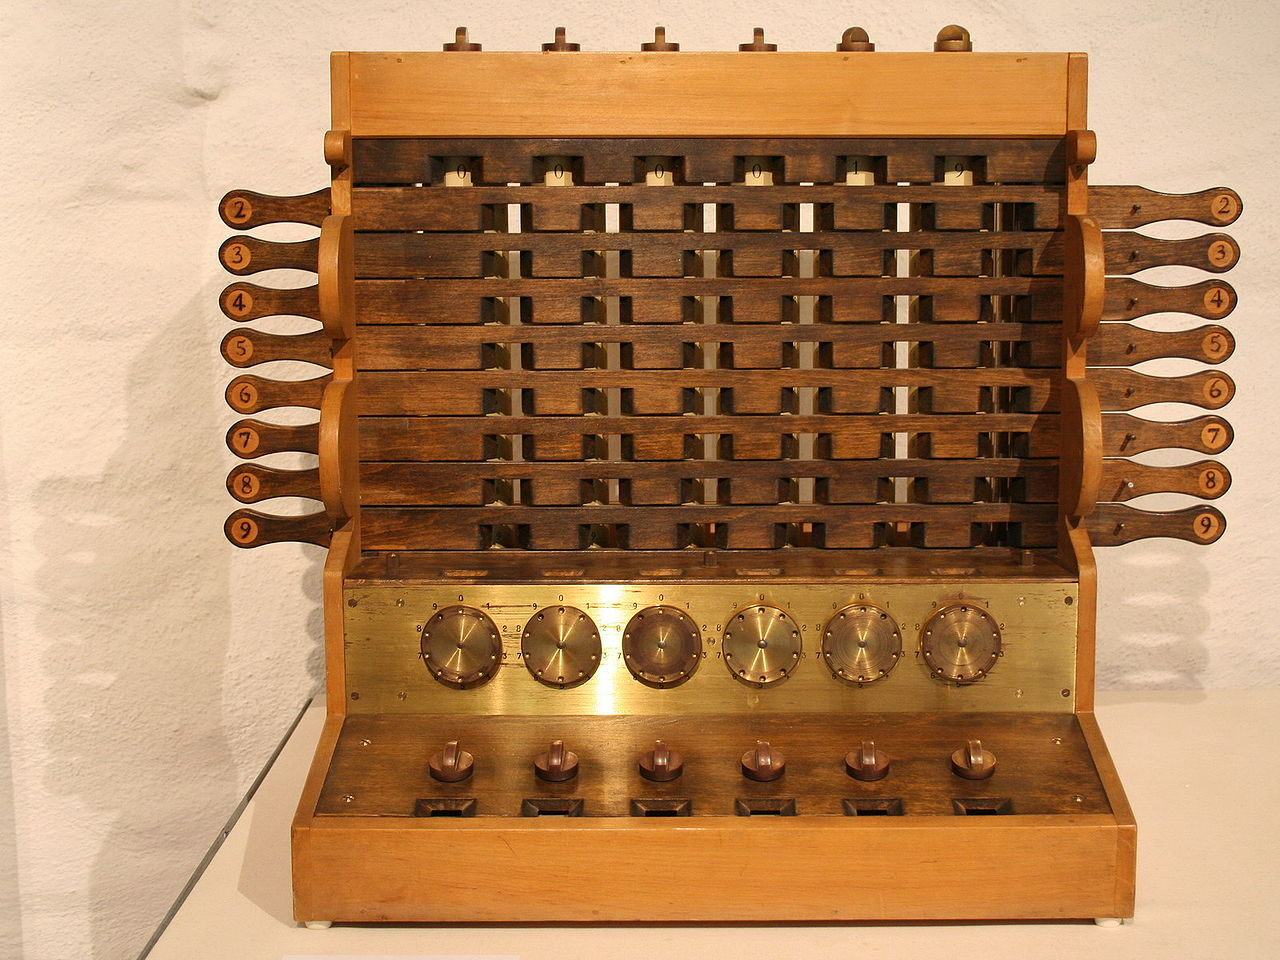
\includegraphics[width=0.5\linewidth]{images/01_calculadora} 

}

\caption{Réplica de la máquina calculadora de Schickard.}\label{fig:calculadora}
\end{figure}

Durante la Revolución Industrial, el rápido crecimiento de la tecnología hizo posible considerar nuevas formas para realizar cálculos matemáticos, tomando provecho de que las máquinas de vapor podían proveer energía para hacer funcionar nuevos mecanismos. En este tiempo, se destacó el matemático británico Charles Babbage, quien diseñó dos tipos de máquinas calculadoras, una para crear tablas de funciones matemáticas (llamada \emph{máquina diferencial}), y otra que concibió como de uso general, capaz de realizar distintas funciones de acuerdo a cómo fuese ``programada'' (\emph{máquina analítica}). La operación de esta máquina era controlada por un patrón de perforaciones hechas sobre una tarjeta que la misma podía leer. Al cambiar el patrón de las perforaciones, se podía cambiar el comportamiento de la máquina para que resuelva diferentes tipos de cálculos. Si bien no llegó a concretar sus diseños en vida y fueron finalizados por otras personas, sentó bases importantes en la historia de la computación.

\begin{figure}

{\centering 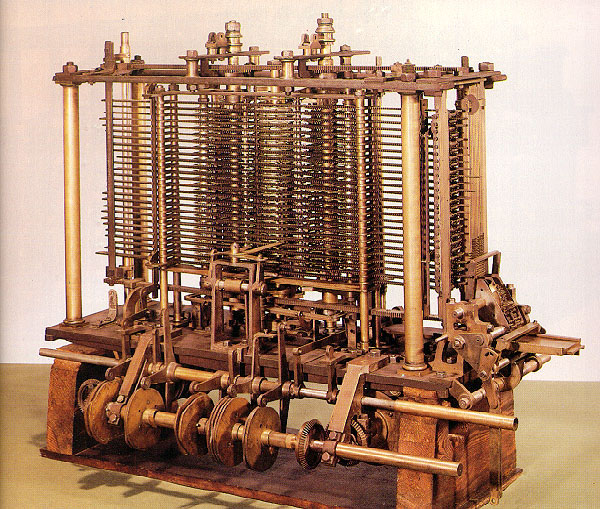
\includegraphics[width=0.5\linewidth]{images/02_maqanalitica} 

}

\caption{La máquina analítica de Babbage.}\label{fig:maqanalitica}
\end{figure}

En 1890, Herman Hollerith utilizó tarjetas perforadas para automatizar la tabulación de datos para el censo de Estados Unidos, y con el fin de comercializar esta tecnología fundó una compañía que terminaría siendo la famosa International Business Machine (IBM). Sin embargo, la visión de Babbage de una computadora programable no se hizo realidad hasta los años 1940, cuando el advenimiento de la electrónica hizo posible superar a los dispositivos mecánicos existentes. El primer prototipo de una computadora electrónica fue armado por John Atanasoff y Clifford Barry en Iowa State College en 1939, que contaba con 300 tubos de vacíos, componentes electrónicos que pueden modificar una señal eléctrica mediante el control del movimiento de los electrones produciendo una respuesta.

\begin{figure}

{\centering 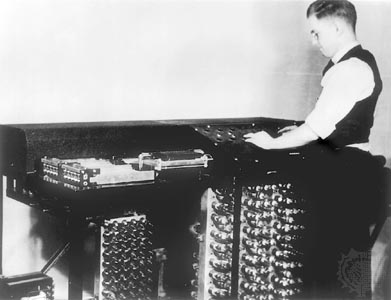
\includegraphics[width=0.5\linewidth]{images/03_berry} 

}

\caption{Réplica de la máquina calculadora de Schickard.}\label{fig:berry}
\end{figure}

La primera computadora electrónica a gran escala fue la ENIAC, \emph{Electronic Numerical Integrator and Computer}, completada por Presper Eckert y John Mauchly en Pennsylvania. Tenía más de 18000 tubos de vacío, ocupaba una sala de 9x15 metros y era controlada conectando ciertos cables en un panel, pero poder programarla resultó ser más difícil de lo que los inventores esperaban. Sin embargo, un gran avance se produjo en 1946, cuando John von Neumann en Princeton propuso que los programas, es decir, las instrucciones para que la máquina opere, y los datos necesarios podrían ser representados y guardados en una memoria interna.

\begin{figure}

{\centering 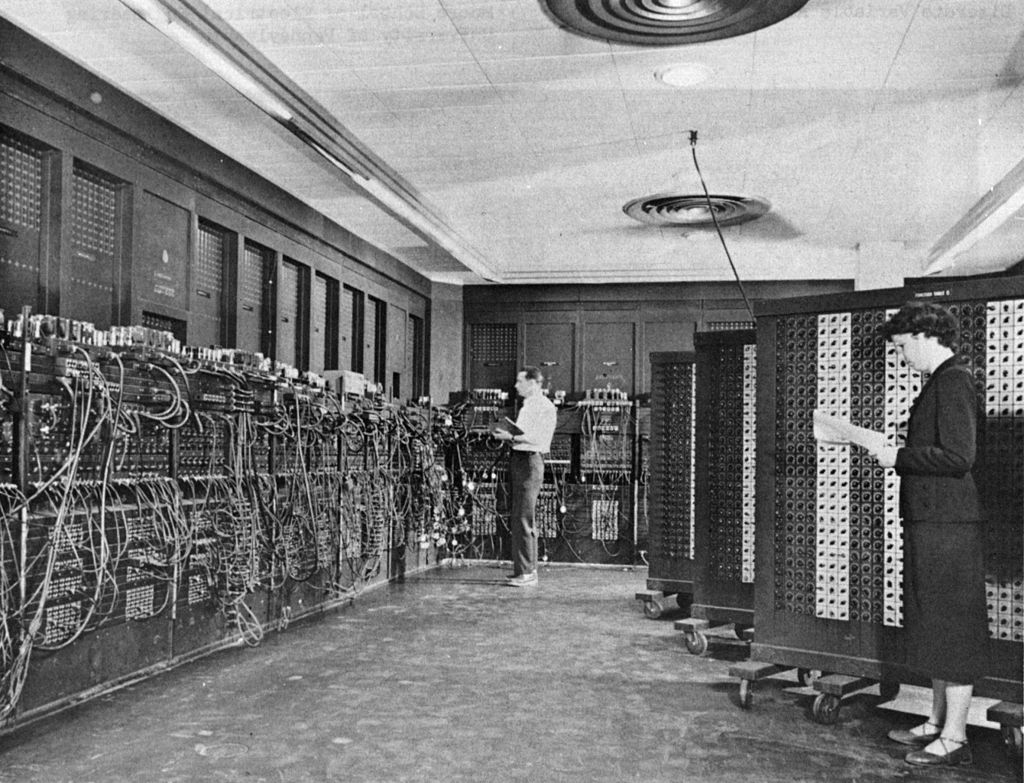
\includegraphics[width=0.5\linewidth]{images/04_eniac} 

}

\caption{La ENIAC en Filadelfia, Pennsylvania.}\label{fig:eniac}
\end{figure}

Desde entonces, la computación ha evolucionado muy rápidamente, con la introducción de nuevos sistemas y conceptos. Algunos historiadores dividen al desarrollo de las computadoras modernas en cuatro generaciones:

\begin{itemize}
\tightlist
\item
  \textbf{Primera generación}: se trata de las computadoras electrónicas que usaban tubos de vacío para su circuito interno como la de Atanasoff.
\item
  \textbf{Segunda generación}: nació a partir de 1947 con el desarrollo del \emph{transistor}, un dispositivo electrónico semiconductor que entrega una señal de salida en respuesta a una señal de entrada, mucho más pequeño que los tubos de vacío y que consumen menos energía eléctrica. Aún así, una computadora podía tener cientos de miles de transistores, ocupando mucho espacio.
\item
  \textbf{Tercera generación}: se inició en 1959 con el desarrollo de un circuito integrado (``chip'') que se trata de una pequeña placa de silicio sobre el cual se imprime un gran número de transistores conectados. La primera computadora de este estilo fue de IBM en 1960.
\item
  \textbf{Cuarta generación}: comenzó en 1975 cuando los avances tecnológicos permitieron construir la unidad entera de procesamiento de una computadora sobre un único chip de silicio. Los procesadores que consisten de un único chip se llaman \emph{microprocesadores} y son utilizados en la mayoría de las computadoras de hoy.
\end{itemize}

\begin{figure}

{\centering 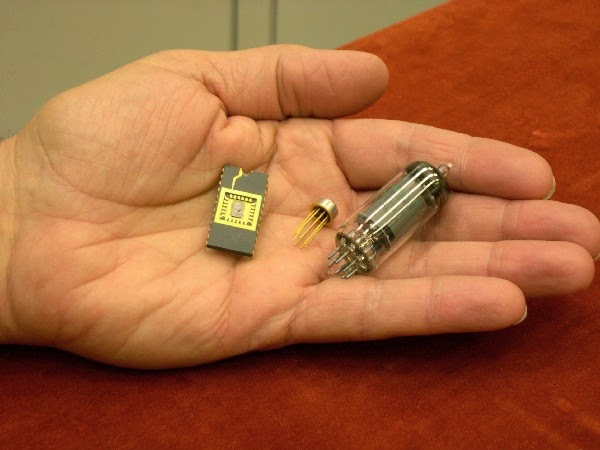
\includegraphics[width=0.5\linewidth]{images/05_tubovacio_transistor_chip} 

}

\caption{De derecha a izquierda: un tubo de vacío, un transistor y un chip.}\label{fig:evolucion}
\end{figure}

\hypertarget{software-y-hardware}{%
\section{Software y hardware}\label{software-y-hardware}}

La computadora en sí misma es sólo una parte de la historia. La máquina física que uno puede comprar y llevar al escritorio de casa es un ejemplo de \textbf{hardware}. Es tangible. Pero para que una computadora pueda cumplir con el propósito general de servir para una variada gama de tareas, debe ser \textbf{programada}. El acto de programar una computadora consiste en proveer un conjunto de instrucciones - un \textbf{programa} - que especifica todos los pasos necesarios para resolver un problema que se le asigna. Estos programas generalmente se conocen como \textbf{software}, y es la conjunción de ambos, hardware y software, la que le da vida a la computación.

\begin{figure}

{\centering 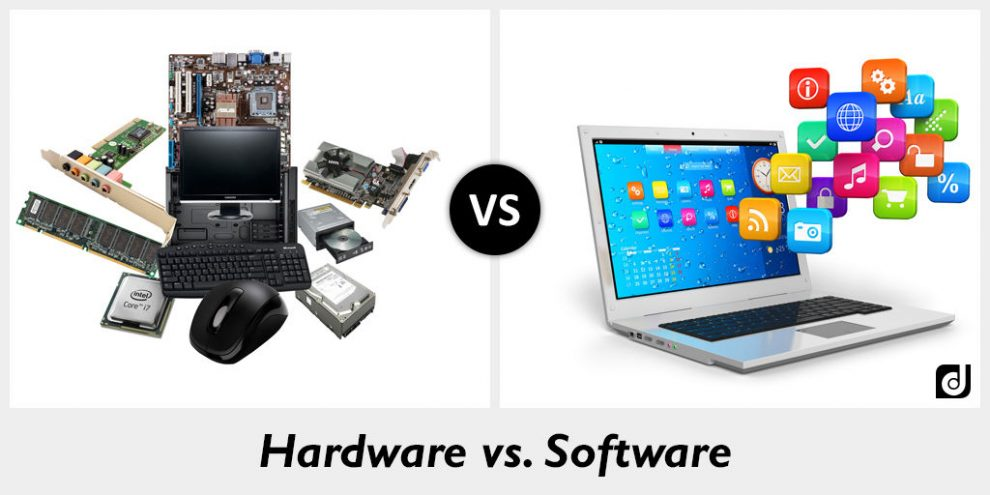
\includegraphics[width=0.5\linewidth]{images/06_hardsoft} 

}

\caption{Representación de la diferencia entre hardware y software.}\label{fig:hardvssoft}
\end{figure}

A diferencia del hardware, el software es una entidad abstracta, intangible. Se trata de una secuencia de pasos simples y operaciones, especificadas en un lenguaje que el hardware puede interpretar. En nuestro \textbf{Taller de Programación} nos concentraremos en el diseño de la solución de un problema y cómo transmitírsela a la computadora para que la misma pueda ejecutarla.

\hypertarget{problemas-algoritmos-y-lenguajes-de-programaciuxf3n}{%
\chapter{Problemas, algoritmos y lenguajes de programación}\label{problemas-algoritmos-y-lenguajes-de-programaciuxf3n}}

Como seres humanos, tenemos incorporada intuitivamente la resolución de problemas cotidianos gracias a nuestra experiencia, y para intentar afrontar un inconveniente, solemos hacer un proceso rápido de selección e intentamos buscar la opción más favorable.

Un \textbf{algoritmo} es una estrategia consistente de un conjunto ordenado de pasos que nos lleva a la solución de un problema o alcance de un objetivo. Un algoritmo cumple con las siguientes características:

\begin{itemize}
\tightlist
\item
  \textbf{Está expresado de manera clara y precisa}: el lector debe poder entender sin ambigüedades cuáles son los pasos involucrados.
\item
  \textbf{Es efectivo}: en el sentido de que sea factible llevar a cabo dichos pasos.
\item
  \textbf{Es finito}: debe arrojar una respuesta o brindar la solución al problema en una cantidad finita de tiempo, es decir, termina luego de un número acotado de pasos.
\end{itemize}

Los algoritmos, así como los problemas que intentan resolver, varían ampliamente en complejidad. Algunos problemas son tan simples que inmediatamente se nos ocurre un algoritmo apropiado para su resolución. Para problemas complejos, en cambio, desarrollar un algoritmo requiere más tiempo y razonamiento, e incluso se pueden originar distintos algoritmos para solucionar un mismo problema.

La resolución computacional de un problema consiste de dos etapas básicas:

\begin{itemize}
\tightlist
\item
  \textbf{Diseño algorítmico}: desarrollar un algoritmo, o elección de uno existente, que resuelva el problema.
\item
  \textbf{Codificación}: expresar un algoritmo en un lenguaje que la computadora pueda interpretar.
\end{itemize}

Al aprender sobre programación, comenzamos enfrentándonos a problemas simples para los cuales la primera etapa parece sencilla, mientras que la codificación se torna dificultosa ya que hay que aprender las reglas del lenguaje de programación. Sin embargo, mientras que con práctica rápidamente podemos ganar facilidad para la escritura de códigos, el diseño algorítmico se torna cada vez más desafiante al encarar problemas más complejos. Es por eso que haremos incapié en el planteo y desarrollo de algoritmos como una etapa fundamental en la programación.

\hypertarget{el-diseuxf1o-algoruxedtmico}{%
\section{El diseño algorítmico}\label{el-diseuxf1o-algoruxedtmico}}

Frente a cada problema, el primer paso es idear una algoritmo para su solución y expresarlo por escrito, por ejemplo, en español, pero adaptando el lenguaje humano a formas lógicas que se acerquen a las tareas que puede realizar una computadora. En programación, el lenguaje artificial e informal que usan los desarrolladores en la confección de algoritmos recibe el nombre de \textbf{pseudocódigo}. Es la herramienta que utilizamos para describir los algoritmos mezclando el lenguaje común con instrucciones de programación. No es en sí mismo un lenguaje de programación, es decir, la computadora no es capaz de entenderlo, sino que el objetivo del mismo es que el programador se centre en la solución lógica y luego lo utilice como guía al escribir el programa.

El pseudocódigo, como cualquier otro lenguaje, está compuesto por:

\begin{itemize}
\tightlist
\item
  Un \textbf{léxico}: conjunto de palabras o frases válidas para escribir las instrucciones
\item
  Una \textbf{sintaxis}: reglas que establecen cómo se pueden combinar las distintas partes
\item
  Una \textbf{semántica}: significado que se les dá a las palabras o frases
\end{itemize}

Además el pseudocódigo, y toda codificación en lenguajes de programación, sigue una \textbf{estructura secuencial}: define una acción o instrucción que sigue a otra en secuencia. Esta estructura puede representarse de la siguiente forma:

\begin{Shaded}
\begin{Highlighting}[]
\NormalTok{ALGORITMO: "Ejemplo"}
\NormalTok{COMENZAR}
\NormalTok{    Acción 1}
\NormalTok{    Acción 2}
\NormalTok{    ...}
\NormalTok{    Acción N}
\NormalTok{FIN}
\end{Highlighting}
\end{Shaded}

Se comienza con un título que describa el problema que el algoritmo resuelve, seguido por la palabra \texttt{COMENZAR}. Luego se detallan las acciones o instrucciones a seguir y se concluye con la palabra \texttt{FIN}. Por ejemplo, si nuestro problema es poner en marcha un auto, el algoritmo para resolverlo puede ser expresado mediante el siguiente pseudocódigo:

\begin{Shaded}
\begin{Highlighting}[]
\NormalTok{ALGORITMO: "Arrancar el auto"}
\NormalTok{COMENZAR}
\NormalTok{    INSERTAR la llave de contacto}
\NormalTok{    UBICAR el cambio en punto muerto}
\NormalTok{    GIRAR la llave hasta la posición de arranque}
\NormalTok{    SI el motor arranca }
\NormalTok{        ENTONCES}
\NormalTok{            DEJAR la llave en posición "encendido"}
\NormalTok{        SI NO}
\NormalTok{            LLAMAR al mecánico}
\NormalTok{    FINSI}
\NormalTok{FIN}
\end{Highlighting}
\end{Shaded}

Es importante destacar la presencia de sangrado (\emph{indentación}), instrucciones, verbos y estructuras de control en el ejemplo anterior.

\hypertarget{codificaciuxf3n-creaciuxf3n-y-ediciuxf3n-de-programas}{%
\section{Codificación: creación y edición de programas}\label{codificaciuxf3n-creaciuxf3n-y-ediciuxf3n-de-programas}}

El algoritmo anterior está presentado en pseudocódigo utilizando el lenguaje español, una opción razonable para compartir esta estrategia entre personas que se comuniquen con este idioma. Claramente, si queremos presentarle nuestro algoritmo a alguien que sólo habla francés, el español ya no sería una buena elección, y mucho menos si queremos presentarle el algoritmo a una computadora.

Para que una computadora pueda entender nuestro algoritmo, debemos traducirlo en un \textbf{lenguaje de programación}: un idioma artificial diseñado para expresar cómputos que puedan ser llevados a cabo por equipos electrónicos, es decir es un medio de comunicación entre el humano y la máquina. Ejemplos de lenguajes de programación son Fortran, BASIC, C++ o Java. En este curso, aprenderemos a utilizar un lenguaje incorporado en el software estadístico SAS: \textbf{IML} (\emph{Interactive Matrix Language}).

\begin{figure}

{\centering 
\includegraphics[width=0.5\linewidth]{images/07_lenguajes} 

}

\caption{Distintos lenguajes de programación y sus logos.}\label{fig:lenguajes}
\end{figure}

Cada una de las acciones que componen al algoritmo son codificadas con una o varias \textbf{instrucciones} o \textbf{sentencias}, expresadas en el lenguaje de programación elegido, y el conjunto de todas ellas constituye un \textbf{programa}. El programa se guarda en un \textbf{archivo} con un nombre generalmente dividido en dos partes por un punto, por ejemplo: \texttt{miPrimerPrograma.sas}. La primera parte es la \textbf{raíz} del nombre con la cual podemos describir el contenido del archivo. La segunda parte es indicativa del uso del archivo, por ejemplo, \texttt{.sas} indica que contiene un programa escrito en el lenguaje de SAS. El proceso general de ingresar o modificar el contenido de un archivo se denomina \textbf{edición}.

Existen distintos tipos de lenguajes de programación que cumplen la función
de intermediarios entre el desarrollador y el hardware. Simplificando esta gran variedad, podemos decir que hay dos grupos generales. Por un lado, se encuentran los lenguajes más próximos a la arquitectura del hardware, denominados \textbf{lenguajes de bajo nivel}, que son más rígidos y complicados de entender para nosotros. Por otro lado, están aquellos más cercanos a los programadores y usuarios, denominados \textbf{lenguajes de alto nivel}, diseñados para que sea fácil para los humanos expresar los algoritmos sin necesidad de entender en detalle cómo hace exactamente el hardware para ejecutarlos. El lenguaje que utilizaremos en este taller, IML, es de alto nivel.

Para que un programa escrito en un lenguaje de alto nivel pueda ser ejecutado, se necesita de \textbf{compiladores} o \textbf{intérpretes} que básicamente lo traducen al lenguaje de bajo nivel que es apropiado para el hardware que se dispone. Un \emph{compilador} toma un programa escrito en lenguaje de alto nivel y produce como resultado un programa escrito en otro lenguaje, que luego puede ser ejecutado, mientras que un \emph{intérprete} traduce y ejecuta simultáneamente.

\hypertarget{errores-de-programaciuxf3n-y-depuraciuxf3n}{%
\section{Errores de programación y depuración}\label{errores-de-programaciuxf3n-y-depuraciuxf3n}}

Tal como el lenguaje humano, los lenguajes de programación tienen su propio vocabulario y su propia sintaxis, que es el conjunto de reglas gramaticales que establecen cómo se pueden combinar las distintas partes del lenguaje. Estas reglas sintácticas determinan que ciertas sentencias están correctamente construidas mientras otras no.

Cuando compilamos un programa, el compilador primero chequea si el mismo es sintácticamente correcto. Si hemos violado alguna regla, mostrará un mensaje de error y debemos editar nuestro programa para corregirlo.

Aunque los errores de sintaxis pueden ser frustrantes, los errores lógicos suelen ser los más problemáticos. Por ejemplo, el programa puede ser compilado sin errores pero arroja resultados incorrectos o ningún resultado. En estos casos hay que revisar el programa para encontrar algún error en la lógica del mismo. Este tipo de errores suelen llamarse \textbf{bugs} y la corrección de los mismos \textbf{debugging} (depuración).

En nuestro recorrido por el taller, seguramente nos enfrentaremos a varias situaciones en las cuales nos parece que el algoritmo es correcto, para luego descubrir que falla porque nos hemos olvidado de considerar alguna situación particular. Si bien esto puede resultar desalentador, forma parte de la práctica cotidiana de todos los programadores.

\begin{figure}

{\centering 
\includegraphics[width=0.5\linewidth]{images/08_bug} 

}

\caption{Encontrando un "bug" en un programa.}\label{fig:bug}
\end{figure}

\hypertarget{resumiendo}{%
\section{Resumiendo}\label{resumiendo}}

A la hora de resolver un problema computacional, seguiremos los siguientes pasos:

\begin{itemize}
\tightlist
\item
  Analizar el problema que vamos a resolver.
\item
  Imaginar una solución (algoritmo).
\item
  Traducir la solución a pseudocódigo.
\item
  Implementar en un lenguaje de programación todo lo analizado.
\item
  Compilar o correr el programa.
\item
  Realizar pruebas de ejecución.
\item
  Corregir los errores que haya.
\end{itemize}

\hypertarget{primeros-pasos-en-sasiml}{%
\chapter{Primeros pasos en SAS/IML}\label{primeros-pasos-en-sasiml}}

\hypertarget{quuxe9-es-sas}{%
\section{Qué es SAS}\label{quuxe9-es-sas}}

\begin{itemize}
\tightlist
\item
  \textbf{SAS} es un paquete de programas orientados al análisis estadístico desarrollado por \textbf{SAS Institute} a finales de los años sesenta.
\item
  Este instituto se inició a finales de los años sesenta como un proyecto en la Universidad de Carolina del Norte para crear un \emph{sistema de análisis estadístico} (\textbf{S}tatistical \textbf{A}nalysis \textbf{S}ystem) originalmente utilizado por los departamentos de Agricultura de algunas universidades.
\item
  En 1976 se convirtió en una compañía y privada y desde entonces tomó relevancia y gran prestigio en la comunidad estadística internacional.
\end{itemize}

\hypertarget{cuxf3mo-instalar-sas}{%
\section{Cómo instalar SAS}\label{cuxf3mo-instalar-sas}}

\begin{itemize}
\tightlist
\item
  SAS no es un software libre y como tal para poder instalarlo y hacer uso del mismo se debe adquirir una licencia.
\item
  Sin embargo, disponen de una versión gratuita pensada para estudiantes universitarios llamada \href{https://www.sas.com/en_us/software/university-edition.html}{SAS University Edition}.
\item
  El link anterior lleva a la página oficial que detalla todos los pasos para poder instalar y usar esta versión gratuita.
\item
  Como alternativa, el siguiente \href{https://www.youtube.com/watch?v=932o9X-8QzM}{video} también provee instrucciones detalladas para Windows.
\end{itemize}

\begin{verbatim}
## PhantomJS not found. You can install it with webshot::install_phantomjs(). If it is installed, please make sure the phantomjs executable can be found via the PATH variable.
\end{verbatim}

\hypertarget{quuxe9-es-sasiml}{%
\section{Qué es SAS/IML}\label{quuxe9-es-sasiml}}

\begin{itemize}
\tightlist
\item
  IML son las siglas de \emph{Interactive Matrix Language}.
\item
  Es decir, IML es un lenguaje de programación que hace foco en la utilización y manejo de vectores y matrices, permiendo hacer con ellos cómputos de alto nivel.
\item
  Permite interactuar con otros procedimientos de SAS, acceder a archivos, y crear gráficos entre otras cosas.
\item
  Incluye un variado conjunto de funciones y operadores para asistir en la programación.
\item
  Leer la guía sobre IML disponible en el Campus Virtual.
\end{itemize}

\hypertarget{cuxf3mo-usar-iml}{%
\section{Cómo usar IML}\label{cuxf3mo-usar-iml}}

\begin{itemize}
\tightlist
\item
  El procedimiento de SAS que implementa este lenguaje se llama de la misma forma, por lo cual todo el código de nuestros programas estará siempre encerrado en bloques del estilo:
\end{itemize}

\begin{Shaded}
\begin{Highlighting}[]
\NormalTok{proc iml;}
\NormalTok{    ...}
\NormalTok{    líneas de código}
\NormalTok{    ...}
\NormalTok{quit;}
\end{Highlighting}
\end{Shaded}

\hypertarget{elementos-para-la-creaciuxf3n-de-algoritmos}{%
\chapter{Elementos para la creación de algoritmos}\label{elementos-para-la-creaciuxf3n-de-algoritmos}}

\hypertarget{procesador-ambiente-y-acciones}{%
\section{Procesador, ambiente y acciones}\label{procesador-ambiente-y-acciones}}

Hemos definido a un algoritmo como una lista de instrucciones que serán traducidas con un lenguaje de programación para ser ejecutadas por computadora. En este sentido, el concepto físico de la máquina o computadora hacer referencia a la necesidad de contar con un \textbf{procesador} para resolver el problema. Se define como \textbf{procesador} a todo agente capaz de entender las órdenes del programa y ejecutarlas.

Para cumplir con esto, el procesador empleará ciertos recursos que forman parte del sistema en el cual se ejecuta el programa. Por ejemplo, utilizará dispositivos de almacenamiento para guardar datos o dispositivos de salida para comunicar el resultado. Todos los elementos disponibles para ser utilizados por el procesador constituyen su \textbf{entorno} o \textbf{ambiente}.

Cada una de las instrucciones que componen el algoritmo modifican el entorno de alguna manera y se denominan \textbf{acciones}.

\hypertarget{ejemplo-1}{%
\subsection{Ejemplo 1}\label{ejemplo-1}}

\begin{itemize}
\tightlist
\item
  \textbf{Problema}: preparar una tortilla de 6 huevos.
\item
  \textbf{Entorno}: una mesa, una hornalla, una sartén, un plato, un tenedor, aceite, una fuente con huevos, un tarro de basura.
\item
  \textbf{Procesador}: un adulto.
\item
  \textbf{Acciones comprensibles por el procesador}: agarrar un huevo, romper un huevo en un plato, batir huevos, poner aceite, poner en la sartén, poner al fuego, retirar del fuego, tirar las cáscaras, encender el fuego.
\end{itemize}

¿Cuál es un algoritmo adecuado para solucionar este problema? Podría ser:

\begin{Shaded}
\begin{Highlighting}[]
\NormalTok{ALGORITMO: "Preparar una tortilla de 6 huevos"}
\NormalTok{COMENZAR}
\NormalTok{    ROMPER seis huevos en un plato}
\NormalTok{    TIRAR las cáscaras en el tacho}
\NormalTok{    BATIR los huevos}
\NormalTok{    CALENTAR aceite en la sartén}
\NormalTok{    PONER el contenido del plato en la sartén}
\NormalTok{    ESPERAR diez minutos}
\NormalTok{    RETIRAR la tortilla del fuego}
\NormalTok{    APAGAR el fuego}
\NormalTok{FIN}
\end{Highlighting}
\end{Shaded}

\hypertarget{ejemplo-2}{%
\subsection{Ejemplo 2}\label{ejemplo-2}}

\begin{itemize}
\tightlist
\item
  \textbf{Problema}: calcular el factorial del número 5.
\item
  \textbf{Entorno}: se dispone de una calculadora común.
\item
  \textbf{Procesador}: un adulto.
\item
  \textbf{Acciones comprensibles por el procesador}: pulsar teclas de la calculadora.
\end{itemize}

¿Cuál es un algoritmo adecuado para solucionar este problema? Podría ser:

\begin{Shaded}
\begin{Highlighting}[]
\NormalTok{ALGORITMO: "Calcular 5!"}
\NormalTok{COMENZAR}
\NormalTok{    PULSAR [ON]}
\NormalTok{    PULSAR [1]}
\NormalTok{    PULSAR [X]}
\NormalTok{    PULSAR [2]}
\NormalTok{    PULSAR [X]}
\NormalTok{    PULSAR [3]}
\NormalTok{    PULSAR [X]}
\NormalTok{    PULSAR [4]}
\NormalTok{    PULSAR [X]}
\NormalTok{    PULSAR [5]}
\NormalTok{    PULSAR [=]}
\NormalTok{    MOSTRAR la pantalla}
\NormalTok{FIN}
\end{Highlighting}
\end{Shaded}

\hypertarget{acciones-primitivas-o-compuestas}{%
\subsection{Acciones primitivas o compuestas}\label{acciones-primitivas-o-compuestas}}

Las acciones del algoritmo pueden clasificarse en función de su complejidad:

\begin{itemize}
\tightlist
\item
  \textbf{Primitivas}: acción sencilla directamente realizable por el procesador.
\item
  \textbf{Compuestas}: compuestas por una sucesión de acciones primitivas.
\end{itemize}

La descripción de un algoritmo en términos de acciones compuestas puede facilitar su comprensión, pero al desarrollar el programa será necesario descomponerlas en acciones primitivas que son las que realmente ejecuta el procesador. Por ejemplo, la acción compuesta en el ejemplo de la tortilla de ``romper seis huevos en un plato'' puede descomponerse en acciones más simples:

\begin{Shaded}
\begin{Highlighting}[]
\NormalTok{REPETIR 6 VECES}
\NormalTok{    TOMAR un huevo}
\NormalTok{    GOLPEAR el huevo para generar una fractura en la cáscara}
\NormalTok{    EJERCER presión sobre la cáscara}
\NormalTok{    DERRAMAR la clara y la yema sobre el plato}
\end{Highlighting}
\end{Shaded}

\hypertarget{objetos-constantes-y-variables}{%
\section{Objetos, constantes y variables}\label{objetos-constantes-y-variables}}

El procesador debe manipular distintas piezas de información que llamamos \textbf{objetos} y que componen al entorno. Según los valores que pueden representar, los objetos pueden ser de tipo:

\begin{itemize}
\tightlist
\item
  \textbf{Numérico}: Representan valores escalares de forma numérica y permiten realizar
  operaciones aritméticas comunes. Ejemplo: 230, 2.
\item
  \textbf{Caracter}: Representan texto, no es posible hacer operaciones
  matemáticas con ellos y van entre comillas. Ejemplo: ``hola'', ``chau123''
\item
  \textbf{Lógicos}: Sólo pueden tener dos valores (\emph{verdadero} o \emph{falso}), ya que representan el resultado de la comparación entre otros objetos.
\end{itemize}

De manera general, al nombre de un objeto se le dice \textbf{identificador}, el cual es una secuencia de caracteres alfanuméricos que sirve para identificarlo a lo largo del algoritmo. Nombrar los objetos hace posible referirse a los mismos, lo cual es esencial para cualquier tipo de procesamiento simbólico.

Ciertos objetos almacenan temporalmente un valor durante la ejecución de un proceso y su contenido puede cambiar mientras corre el programa. Este tipo de objetos recibien el nombre de \textbf{variables}. Por ejemplo, en un programa creado para un comercio puede existir un objeto llamado \emph{stock} (identificador) de tipo numérico que reprsenta la cantidad de artículos disponibles y cuyo valor se modifica cada vez que se registra una nueva venta. Podemos pensar a una variable como una caja que contiene una etiqueta con su identificador y un valor, por ejemplo, una simple letra (como ``k'', tipo caracter) o un valor numérico (como ``2019'', tipo numérico).

\begin{figure}

{\centering 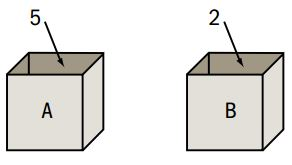
\includegraphics[width=0.5\linewidth]{images/09_cajas} 

}

\caption{Las variables A y B contienen a los valores 5 y 2 respectivamente.}\label{fig:cajas}
\end{figure}

Si un objeto tiene siempre necesariamente un valor fijo, se dice que es una \textbf{constante}. El valor es siempre el mismo para cualquier ejecución del programa, es decir, no puede cambiar de una ejecución a otra. Son ejemplos de constantes el número de meses del año, las constantes matemáticas tales como el número π, los factores de conversión de unidades de medida, etc. Las constantes pueden usarse literalmente, es decir, usando explícitamente el valor, o también a través de un objeto que asocie un identificador al valor constante (por ejemplo, asociar el nombre ``pi'' a la constante 3.14159265).

\hypertarget{declaraciuxf3n-de-variables-y-constantes}{%
\subsection{Declaración de variables y constantes}\label{declaraciuxf3n-de-variables-y-constantes}}

Al expresar nuestros algoritmos en pseudocódigo tomaremos la costumbre de declarar al inicio del mismo las variables y constantes necesarias para resolver el problema, explicitando su identificador y determinando el tipo de valor que guarda. Muchos lenguajes de programación utilizan esta declaración para reservar en la memoria de la computadora un espacio para almacenar la información correspondiente de manera adecuada.

\textbf{En IML}. IML es un lenguaje dinámico que no requiere la declaración previa de las variables que serán utilizadas, sino que estas pueden definirse dinámicamente a lo largo del programa. Por eso, incluiremos declaración de variables y constantes sólo en los algoritmos.

\hypertarget{acciuxf3n-de-asignaciuxf3n}{%
\subsection{Acción de asignación}\label{acciuxf3n-de-asignaciuxf3n}}

Para hacer que una variable guarde un determinado valor se recurre a una \textbf{acción de asignación}. Mediante asignaciones podemos dar valores iniciales a las variables, modificar el valor que tenían hasta el momento o guardar en ellas resultados intermedios o finales del algoritmo.

En pseudocódigo expresaremos a la asignación como se muestra en estos ejemplos:

\begin{Shaded}
\begin{Highlighting}[]
\NormalTok{lugarNacimiento \textless{}{-} "Bombal"}
\NormalTok{pesoNacimiento \textless{}{-} 3.423}
\end{Highlighting}
\end{Shaded}

Si intervienen variables en la expresión a la derecha de una acción de asignación, se usará el valor que tenga la variable en ese momento. Por ejemplo, la siguiente secuencia de acciones en un algoritmo:

\begin{Shaded}
\begin{Highlighting}[]
\NormalTok{meses \textless{}{-} 2}
\NormalTok{dias \textless{}{-} meses}
\NormalTok{meses \textless{}{-} 7}
\NormalTok{saldo \textless{}{-} meses}
\end{Highlighting}
\end{Shaded}

resultará en que las variables \texttt{meses}, \texttt{dias} y \texttt{saldo} tengan almacenados los valores 7, 2 y 7 respectivamente. Un caso particular se da cuando a una variable se le asigna el valor de una operación de la que forma parte la misma variable. Por ejemplo:

\begin{Shaded}
\begin{Highlighting}[]
\NormalTok{dias \textless{}{-} dias + 30}
\end{Highlighting}
\end{Shaded}

\textbf{En IML}. La asignación se realiza a través del símbolo =. El código para el ejemplo anterior es:

\begin{Shaded}
\begin{Highlighting}[]
\NormalTok{proc iml;}
\NormalTok{    meses = 2;}
\NormalTok{    dias = meses;}
\NormalTok{    meses = 7;}
\NormalTok{    saldo = meses;}
\NormalTok{    print meses dias saldo;}
\NormalTok{quit;}
\end{Highlighting}
\end{Shaded}

\hypertarget{operadores}{%
\section{Operadores}\label{operadores}}

El desarrollo de un algoritmo involucra la necesidad de efectuar operaciones de distinto tipo: suma, resta, concatenación, procesos lógicos, etc. Los elementos que describen el tipo de operación a realizar entre dos objetos se denominan \textbf{operadores}.

\hypertarget{operadores-aritmuxe9ticos}{%
\subsection{Operadores aritméticos}\label{operadores-aritmuxe9ticos}}

Permiten realizar operaciones matemáticas con objetos de tipo numérico.

\begin{table}

\caption{\label{tab:unnamed-chunk-12}Signos para operadores aritméticos que se pueden utilizar en el pseudocódigo.}
\centering
\begin{tabular}[t]{l|l}
\hline
Signo & Significado\\
\hline
+ & Suma\\
\hline
- & Resta\\
\hline
* & Multiplicación\\
\hline
/ & División\\
\hline
** & Potenciación\\
\hline
MOD & Resto de la división entera\\
\hline
\end{tabular}
\end{table}

Los operadores aritméticos actúan con un orden de prioridad establecido, tal como estamos acostumbrados en matemática. Las expresiones entre paréntesis se evalúan primero. Si hay paréntesis anidados se evalúan desde adentro hacia afuera. Dentro de una misma expresión, los operadores se evalúan en este orden:

\begin{enumerate}
\def\labelenumi{\arabic{enumi}.}
\tightlist
\item
  Potenciación
\item
  Multiplicación, división, módulo
\item
  Suma, resta
\end{enumerate}

Si la expresión presenta operadores con igual nivel de prioridad, se evalúan de izquierda a derecha. Ejemplos:

\begin{Shaded}
\begin{Highlighting}[]
\NormalTok{4 + 2 * 4 = 12}
\NormalTok{23 * 2 / 5 = 9.2}
\NormalTok{3 + 5 * (10 {-} (2 + 4)) = 23}
\NormalTok{2.1 * 1.5 + 12.3 = 15.45}
\NormalTok{2.1 * (1.5 + 12.3) = 28.98}
\NormalTok{1 MOD 4 = 1}
\NormalTok{8 * (7 {-} 6 + 5) MOD (1 + 8 / 2) {-} 1 = ...}
\end{Highlighting}
\end{Shaded}

\textbf{En IML}. Se utilizan los mismos símbolos, excepto para el operador módulo, cuya sintaxis es, por ejemplo, \texttt{mod(7,\ 4)} si se quiere obtener el resto de la división de 7 por 4.

\hypertarget{operadores-relacionales}{%
\subsection{Operadores relacionales}\label{operadores-relacionales}}

Sirven para comparar dos valores de cualquier tipo y dan como resultado un valor lógico: \emph{verdadero} (``V'') o \emph{falso} (``F'').

\begin{table}

\caption{\label{tab:unnamed-chunk-14}Signos para operadores lógicos que se pueden utilizar en el pseudocódigo.}
\centering
\begin{tabular}[t]{l|l}
\hline
Signo & Significado\\
\hline
> & Mayor que\\
\hline
< & Menor que\\
\hline
>= & Mayor o igual que\\
\hline
<= & Menor o igual que\\
\hline
= & Igual a\\
\hline
\textasciicircum{}= & Distinto a\\
\hline
\end{tabular}
\end{table}

Ejemplos:

\begin{table}

\caption{\label{tab:unnamed-chunk-15}Ejemplos de la utilización de operadores relacionales.}
\centering
\begin{tabular}[t]{l|l}
\hline
Operación relacional & Resultado\\
\hline
5 > 3 & verdadero\\
\hline
5 <= 3 & falso\\
\hline
3 * 4 = 10 + 2 & verdadero\\
\hline
3 * 4 \textasciicircum{}= 15 - 4 & verdadero\\
\hline
\end{tabular}
\end{table}

\textbf{En IML}. Se usan estos mismos símbolos.

\hypertarget{operadores-luxf3gicos}{%
\subsection{Operadores lógicos}\label{operadores-luxf3gicos}}

Mientras que los operadores relacionales comparan cualquier tipo de valores, los operadores lógicos sólo toman operandos de tipo lógico y producen también un resultado lógico. Los operadores lógicos que utilizaremos son \textbf{Y}, \textbf{O} y \textbf{NO}.

\begin{itemize}
\tightlist
\item
  El operador lógico \textbf{Y} devuelve un valor \textbf{verdadero} sólo si son verdaderas las dos expresiones que vincula. Ejemplo: (3 \textgreater{} 2) Y (3 \textgreater{} 5) ≡ V Y F ≡ F.
\item
  El operador lógico \textbf{O} devuelve un valor \textbf{verdadero} si al menos una de las dos expresiones que vincula es verdadera. Ejemplo: (3 \textgreater{} 2) O (3 \textgreater{} 5) ≡ V O F ≡ V.
\item
  El operador lógico \textbf{NO}, niega un valor lógico, es decir, devuelve el opuesto. Ejemplo: NO (3 \textgreater{} 2) ≡ NO V ≡ F.
\end{itemize}

Las \textbf{tablas de la verdad} se utilizan para mostrar el resultado de los distintos tipos de operaciones lógicas:

\begin{table}

\caption{\label{tab:unnamed-chunk-16}Tabla de la verdad.}
\centering
\begin{tabular}[t]{l|l|l|l}
\hline
Valor1 & Operador & Valor2 & Resultado\\
\hline
F & Y & F & F\\
\hline
F & Y & V & F\\
\hline
V & Y & F & F\\
\hline
V & Y & V & V\\
\hline
F & O & F & F\\
\hline
F & O & V & V\\
\hline
V & O & F & V\\
\hline
V & O & V & V\\
\hline
 & NO & F & V\\
\hline
 & NO & V & F\\
\hline
\end{tabular}
\end{table}

Ejemplo: expresar con símbolos la expresión ``x no es igual a 2 ni a 3''.

Expresiones correctas:

\begin{Shaded}
\begin{Highlighting}[]
\NormalTok{x \^{}= 2 Y x \^{}= 3}
\NormalTok{NO(x = 2 O x = 3)}
\end{Highlighting}
\end{Shaded}

Expresión incorrecta:

\begin{Shaded}
\begin{Highlighting}[]
\NormalTok{x \^{}= 2 O x \^{}= 3}
\end{Highlighting}
\end{Shaded}

Las Leyes de Morgan nos ayudan a trabajar en este tipo de casos:

\begin{itemize}
\tightlist
\item
  \textbf{NO (Valor1 O Valor2)} \emph{es equivalente a} \textbf{NO Valor1 Y NO Valor2}
\item
  \textbf{NO (Valor1 Y Valor2)} \emph{es equivalente a} \textbf{NO Valor1 O NO Valor2}
\end{itemize}

Otra consideración es que expresiones que tienen sentido en matemática, pueden no tenerlo en programación y deben ser re estructuradas en las formas antes vistas. Por ejemplo, si queremos evaluar si es \texttt{V} o \texttt{F}la expresión \texttt{0\ \textless{}\ x\ \textless{}\ 10}, debemos evaluar \texttt{0\ \textless{}\ x\ Y\ x\ \textless{}\ 10}.

\textbf{En IML}. El operador Y se escribe como ``\&'', el operador O es ``\textbar{}'' y el operador NO es ``\^{}''.

\hypertarget{entrada-y-salida-de-informaciuxf3n}{%
\section{Entrada y salida de información}\label{entrada-y-salida-de-informaciuxf3n}}

En la resolución de problemas puede ser necesario requerir que un usuario provea información, y registrar la misma como un valor que debe ser asignado a una variable. Para esto podemos utilizar la acción \texttt{LEER} dentro del algoritmo. Cuando deseamos mostrar un resultado en un mensaje empleamos la acción \texttt{ESCRIBIR}. Las palabras o frases literales que se desean mostrar en el mensaje deben estar encerradas entre comillas porque son cadenas de texto, mientras que si se desea mostrar el valor de una variable se debe escribir su identificador sin comillas.

\textbf{En IML}. La acción \texttt{LEER} la ejecutaremos mediante la asignación directa de un valor a una variable a través del símbolo ``=''. La acción \texttt{ESCRIBIR} será ejecutada a través de la sentencia \texttt{print} para obtener un resultado en la ventana de Output.

\hypertarget{empleo-de-comentarios-en-el-algoritmo}{%
\section{Empleo de comentarios en el algoritmo}\label{empleo-de-comentarios-en-el-algoritmo}}

A medida que los algoritmos se hacen más complejos, suele ser necesario añadir en el mismo ciertos comentarios que no son acciones que el procesador debe ejecutar, sino que cumplen con la función de explicar alguna característica del algoritmo a otra persona que lo esté leyendo (o a uno mismo si lo leemos nuevamente en el futuro).

Cada vez que deseemos incluir un comentario, lo haremos en una línea que comience con el símbolo ``\textbackslash\textbackslash{}''.

\hypertarget{ejemplo}{%
\section{Ejemplo}\label{ejemplo}}

Los conceptos enunciados anteriormente pueden verse ejemplificados en el siguiente algoritmo para calcular el área de un círculo

\begin{Shaded}
\begin{Highlighting}[]
\NormalTok{ALGORITMO: "Calcular área de un círculo"}
\NormalTok{COMENZAR}
\NormalTok{    CONSTANTE numérica pi}
\NormalTok{    VARIABLE numérica radio, area}
\NormalTok{    pi \textless{}{-} 3.1416}
\NormalTok{    LEER radio}
\NormalTok{    area \textless{}{-} pi * radio ** 2}
\NormalTok{    ESCRIBIR "El área del círculo es " area}
\NormalTok{FIN}
\end{Highlighting}
\end{Shaded}

\textbf{En IML}:

\begin{Shaded}
\begin{Highlighting}[]
\NormalTok{/* PROGRAMA: Calcular área de un círculo */}
\NormalTok{proc iml;}
\NormalTok{    pi = 3.14159265358979;}
\NormalTok{    radio = 5;}
\NormalTok{    area = pi * radio ** 2;}
\NormalTok{    print "El área del círculo es " area;}
\NormalTok{quit;}
\end{Highlighting}
\end{Shaded}

\hypertarget{estructuras-de-control}{%
\chapter{Estructuras de Control}\label{estructuras-de-control}}

Como mencionamos anteriormente, un algoritmo está compuesto por una sucesión ordenada de comandos que se ejecutan uno detrás de otro. Sin embargo, con frecuencia es necesario recurrir a comandos especiales que alteran o controlan el flujo de las acciones. Por lo tanto, decimos que existen distintas \textbf{estructuras de control} que organizan a los algoritmos y que pueden clasificarse en \textbf{secuenciales}, \textbf{condicionales} e \textbf{iterativas}.

\hypertarget{estructuras-de-control-secuenciales}{%
\section{Estructuras de control secuenciales}\label{estructuras-de-control-secuenciales}}

Las estructuras secuenciales están compuestas por un número definido de acciones que se ubican en un orden específico y se suceden una tras otra. Los ejemplos que hemos discutido anteriormente están conformados por este tipo de estructura.

\hypertarget{estructuras-de-control-condicionales}{%
\section{Estructuras de control condicionales}\label{estructuras-de-control-condicionales}}

El curso de acción depende del resultado de la comparación una variable con un valor, que puede ser una constante u otra variable. Existen tres tipos de estructuras condicionales: \textbf{simples}, \textbf{dobles} y \textbf{múltiples}.

\hypertarget{estructuras-condicionales-simples}{%
\subsection{Estructuras condicionales simples}\label{estructuras-condicionales-simples}}

Representan una toma de decisión y se describen con la siguiente sintaxis:

\begin{Shaded}
\begin{Highlighting}[]
\NormalTok{SI \textless{}condición\textgreater{} ENTONCES}
\NormalTok{    Acción/es}
\NormalTok{FIN SI}
\end{Highlighting}
\end{Shaded}

La palabra \texttt{SI} indica el comando de comparación, \texttt{\textless{}condición\textgreater{}} indica la condición a evaluar y \texttt{Acción/es} son las instrucciones que se realizarán sólo si se cumple la condición. Si la condición no se verifica, no se ejecuta ninguna acción y el algoritmo sigue su estructura secuencial a continuación del \texttt{FIN\ SI}.

En el siguiente ejemplo utilizaremos esta estructura para determinar si una persona es mayor de edad o no.

\begin{Shaded}
\begin{Highlighting}[]
\NormalTok{ALGORITMO: "Determinar mayoría de edad"}
\NormalTok{COMENZAR}
\NormalTok{    VARIABLE numérica edad}
\NormalTok{    LEER edad}
\NormalTok{    SI edad \textgreater{}= 18 ENTONCES}
\NormalTok{        ESCRIBIR "Es mayor de edad"}
\NormalTok{    FIN SI}
\NormalTok{FIN}
\end{Highlighting}
\end{Shaded}

\textbf{En IML}. Usamos la estructura \texttt{if\ ...\ then\ ...;}:

\begin{Shaded}
\begin{Highlighting}[]
\NormalTok{/* PROGRAMA: Determinar mayoría de edad */}
\NormalTok{proc iml;}
\NormalTok{    edad = 19;}
\NormalTok{    if edad \textgreater{}= 18 then print "Es mayor de edad";}
\NormalTok{quit;}
\end{Highlighting}
\end{Shaded}

Si necesitamos ejecutar más de una acción al cumplirse la condición evaluada, debemos encerrarlas dentro de un bloque \texttt{do}, que siempre termina con un \texttt{end}:

\begin{Shaded}
\begin{Highlighting}[]
\NormalTok{/* PROGRAMA: Determinar mayoría de edad */}
\NormalTok{proc iml;}
\NormalTok{    edad = 19;}
\NormalTok{    if edad \textgreater{}= 18 then do;}
\NormalTok{        print "Es mayor de edad";}
\NormalTok{        print "Su edad es " edad " años";}
\NormalTok{    end;}
\NormalTok{quit;}
\end{Highlighting}
\end{Shaded}

\hypertarget{estructuras-condicionales-dobles}{%
\subsection{Estructuras condicionales dobles}\label{estructuras-condicionales-dobles}}

Este tipo de estructura añade una acción a ejecutarse en el caso de que la condición evaluada no se verifique. La sintaxis es:

\begin{Shaded}
\begin{Highlighting}[]
\NormalTok{SI \textless{}condición\textgreater{} }
\NormalTok{    ENTONCES}
\NormalTok{        Acción/es}
\NormalTok{    SI NO}
\NormalTok{        Acción/es}
\NormalTok{FIN SI}
\end{Highlighting}
\end{Shaded}

La palabra \texttt{ENTONCES} antecede a las acciones que se realizan si se cumple la condición y \texttt{SI\ NO} a las que se realizan si no se verifica la misma. Podemos ampliar el ejemplo anterior para que el algorimo indique también si la persona es menor de edad:

\begin{Shaded}
\begin{Highlighting}[]
\NormalTok{ALGORITMO: "Determinar mayoría de edad"}
\NormalTok{COMENZAR}
\NormalTok{    VARIABLE numérica edad}
\NormalTok{    LEER edad}
\NormalTok{    SI edad \textgreater{}= 18 }
\NormalTok{        ENTONCES}
\NormalTok{            ESCRIBIR "Es mayor de edad"}
\NormalTok{        SI NO}
\NormalTok{            ESCRIBIR "Es menor de edad"}
\NormalTok{    FIN SI}
\NormalTok{FIN}
\end{Highlighting}
\end{Shaded}

\textbf{En IML}.

\begin{Shaded}
\begin{Highlighting}[]
\NormalTok{proc iml;}
\NormalTok{    edad = 17;}
\NormalTok{    if edad \textgreater{}= 18 then print "Es mayor de edad";}
\NormalTok{    else print "Es menor de edad";}
\NormalTok{quit;}
\end{Highlighting}
\end{Shaded}

Nuevamente, si necesitamos ejecutar múltiples acciones debemos encerrarlas dentro de un bloque \texttt{do}:

\begin{Shaded}
\begin{Highlighting}[]
\NormalTok{proc iml;}
\NormalTok{    edad = 19;}
\NormalTok{    if edad \textgreater{}= 18 then do;}
\NormalTok{        print "Es mayor de edad";}
\NormalTok{        print "Su edad es " edad " años";}
\NormalTok{    end;}
\NormalTok{    else do;}
\NormalTok{        print "Es menor de edad";}
\NormalTok{        print "Requerir ingreso acompañado";}
\NormalTok{    end;}
\NormalTok{quit;}
\end{Highlighting}
\end{Shaded}

\hypertarget{estructuras-condicionales-muxfaltiples-o-anidadas}{%
\subsection{Estructuras condicionales múltiples o anidadas}\label{estructuras-condicionales-muxfaltiples-o-anidadas}}

Permiten combinar varias estructuras condicionales para establecer controles más complejos sobre el flujo de las acciones, representando una toma de decisión múltiple. Podemos ejemplificar la sintaxis de la siguiente forma:

\begin{Shaded}
\begin{Highlighting}[]
\NormalTok{SI \textless{}condición\textgreater{} }
\NormalTok{    ENTONCES}
\NormalTok{        Acción/es}
\NormalTok{    SI NO}
\NormalTok{        SI \textless{}condición\textgreater{} }
\NormalTok{            ENTONCES}
\NormalTok{                Acción/es}
\NormalTok{            SI NO}
\NormalTok{                Acción/es}
\NormalTok{        FIN SI}
\NormalTok{FIN SI}
\end{Highlighting}
\end{Shaded}

Imaginemos que el ejemplo anterior de la mayoría de edad se da en el contexto de la entrada a una exhibición, donde los mayores de edad pueden ingresar pero los menores sólo pueden hacerlo si tienen la autorización de un adulto a cargo. Podemos plantear el siguiente algoritmo para determinar si una persona puede ingresar o no:

\begin{Shaded}
\begin{Highlighting}[]
\NormalTok{ALGORITMO: "Determinar ingreso"}
\NormalTok{COMENZAR}
\NormalTok{    VARIABLE numérica edad}
\NormalTok{    VARIABLE caracter autorizacion}
\NormalTok{    LEER edad}
\NormalTok{    SI edad \textgreater{}= 18 }
\NormalTok{        ENTONCES}
\NormalTok{            ESCRIBIR "Permitir ingreso"}
\NormalTok{        SI NO}
\NormalTok{            LEER autorizacion}
\NormalTok{            SI autorizacion = "OK" }
\NormalTok{                ENTONCES}
\NormalTok{                    ESCRIBIR "Permitir ingreso"}
\NormalTok{                SI NO}
\NormalTok{                    ESCRIBIR "Denegar ingreso"}
\NormalTok{            FIN SI}
\NormalTok{    FIN SI}
\NormalTok{FIN}
\end{Highlighting}
\end{Shaded}

\begin{Shaded}
\begin{Highlighting}[]
\NormalTok{/* PROGRAMA: Determinar ingreso */}
\NormalTok{proc iml;}
\NormalTok{    edad = 16;}
\NormalTok{    autorizacion = "OK";}
\NormalTok{    if edad \textgreater{}= 18 then print "Permitir ingreso";}
\NormalTok{    else do;}
\NormalTok{        if autorizacion = "OK" then print "Permitir ingreso";}
\NormalTok{        else print "Denegar ingreso";}
\NormalTok{    end;}
\NormalTok{quit;}
\end{Highlighting}
\end{Shaded}

\hypertarget{estructuras-de-control-iterativas}{%
\section{Estructuras de control iterativas}\label{estructuras-de-control-iterativas}}

Las estructuras de control iterativas son útiles cuando la solución de un problema requiere que se ejecute repetidamente un determinado conjunto de acciones. El número de veces que se debe repetir dicha secuencia de acciones puede ser fijo o variable dependiendo de algún dato en el algoritmo.

\hypertarget{estructuras-de-control-iterativas-con-un-nuxfamero-fijo-de-iteraciones}{%
\subsection{Estructuras de control iterativas con un número fijo de iteraciones}\label{estructuras-de-control-iterativas-con-un-nuxfamero-fijo-de-iteraciones}}

Se aplican cuando se conoce de antemano el número exacto de veces que se debe repetir una secuencia de acciones. Por ejemplo, si deseamos mostrar en pantalla la tabla de multiplicar del número 8 completa podríamos hacer:

\begin{Shaded}
\begin{Highlighting}[]
\NormalTok{ALGORIMO: "Mostrar tabla del 8"}
\NormalTok{COMENZAR}
\NormalTok{    VARIABLE numérica resultado}
\NormalTok{    resultado \textless{}{-} 8 * 1}
\NormalTok{    ESCRIBIR "8 x 1 = ", resultado}
\NormalTok{    resultado \textless{}{-} 8 * 2}
\NormalTok{    ESCRIBIR "8 x 2 = ", resultado}
\NormalTok{    resultado \textless{}{-} 8 * 3}
\NormalTok{    ESCRIBIR "8 x 3 = ", resultado}
\NormalTok{    ...}
\NormalTok{    resultado \textless{}{-} 8 * 10}
\NormalTok{    ESCRIBIR "8 x 10 = ", resultado}
\NormalTok{FIN}
\end{Highlighting}
\end{Shaded}

Es evidente que hay dos acciones que se repiten a través de todo el algorimo con una leve variación en el número por el cual se está multiplicando al 8. Esto puede resumirse así:

\begin{Shaded}
\begin{Highlighting}[]
\NormalTok{ALGORIMO: "Mostrar tabla del 8"}
\NormalTok{COMENZAR}
\NormalTok{    VARIABLE numérica resultado}
\NormalTok{    PARA i DESDE 1 HASTA 10 HACER}
\NormalTok{        resultado \textless{}{-} 8 * i}
\NormalTok{        ESCRIBIR "8 x " i " = " resultado}
\NormalTok{    FIN PARA}
\NormalTok{FIN}
\end{Highlighting}
\end{Shaded}

De manera general, la sintaxis para este tipo de estructuras es:

\begin{Shaded}
\begin{Highlighting}[]
\NormalTok{PARA \textless{}variable\textgreater{} DESDE \textless{}valor1\textgreater{} HASTA \textless{}valor2\textgreater{} CON PASO \textless{}valor3\textgreater{} HACER}
\NormalTok{    Acción/es}
\NormalTok{FIN PARA}
\end{Highlighting}
\end{Shaded}

Dado un valor inicial \texttt{\textless{}valor1\textgreater{}} asignado a la \texttt{\textless{}variable\textgreater{}}, esta se irá aumentando o disminuyendo según el paso \texttt{\textless{}valor3\textgreater{}} hasta llegar a tomar el valor \texttt{\textless{}valor3\textgreater{}}. Si no se indica el paso se asume que la variable aumenta de uno en uno.

\textbf{En IML}.

\begin{Shaded}
\begin{Highlighting}[]
\NormalTok{/* PROGRAMA: Mostrar tabla del 8 */}
\NormalTok{proc iml;}
\NormalTok{    do i = 1 to 10;}
\NormalTok{        resultado = 8 * i;}
\NormalTok{        print "8 x " i " = " resultado;}
\NormalTok{    end;}
\NormalTok{quit;}
\end{Highlighting}
\end{Shaded}

\hypertarget{estructuras-de-control-iterativas-con-un-nuxfamero-indeterminado-de-iteraciones}{%
\subsection{Estructuras de control iterativas con un número indeterminado de iteraciones}\label{estructuras-de-control-iterativas-con-un-nuxfamero-indeterminado-de-iteraciones}}

En otras circunstancias se puede necesitar repetir un bloque de acciones sin conocer con exactitud cuántas veces, si no que esto depende de algún otro aspecto del ALGORITMO. Las iteraciones pueden continuar \emph{mientras que} o \emph{hasta que} se verifique alguna condición, dando lugar a dos tipos de estructuras.

\hypertarget{mientras-que}{%
\subsubsection{Mientras que}\label{mientras-que}}

El conjunto de sentencias se repite mientras que se siga evaluando como \texttt{VERDADERO} una condición declarada al inicio del bloque. Cuando la condición ya no se cumple, el proceso deja de ejecutarse. La sintaxis es:

\begin{Shaded}
\begin{Highlighting}[]
\NormalTok{MIENTRAS QUE \textless{}condición\textgreater{} HACER}
\NormalTok{    Acción/es}
\NormalTok{FIN MIENTRAS}
\end{Highlighting}
\end{Shaded}

El siguiente ejemplo describe el algoritmo para escribir los múltiplos de 8 menores a 150 utilizando este tipo de estructura:

\begin{Shaded}
\begin{Highlighting}[]
\NormalTok{ALGORITMO: "Múltiplos de 8 menores a 150"}
\NormalTok{COMENZAR}
\NormalTok{    VARIABLE numérica multiplo}
\NormalTok{    multiplo \textless{}{-} 8}
\NormalTok{    MIENTRAS QUE multiplo \textless{} 150 HACER}
\NormalTok{        ESCRIBIR multiplo}
\NormalTok{        multiplo \textless{}{-} multiplo + 8}
\NormalTok{    FIN MIENTRAS}
\NormalTok{FIN}
\end{Highlighting}
\end{Shaded}

Observaciones:

\begin{itemize}
\tightlist
\item
  La evaluación de la condición se lleva a cabo antes de cada iteración, incluyendo la primera. Si la condición es \texttt{FALSO} inicialmente, entonces las acciones en el cuerpo de la estructura no se ejecutan nunca.
\item
  La evaluación de la condición \textbf{sólo} se lleva a cabo al inicio de cada iteración. Si la condición se vuelve \texttt{FALSO} en algún punto durante la ejecución de un bloque, el programa no lo nota hasta que se termine de ejecutar el bloque y la condición sea evaluada antes de comenzar la próxima iteración.
\end{itemize}

\textbf{En IML}.

\begin{Shaded}
\begin{Highlighting}[]
\NormalTok{/* PROGRAMA: Múltiplos de 8 menores a 150 */}
\NormalTok{proc iml;}
\NormalTok{    multiplo = 8;}
\NormalTok{    do while (multiplo \textless{} 150);}
\NormalTok{        print multiplo;}
\NormalTok{        multiplo = multiplo + 8;}
\NormalTok{    end;}
\NormalTok{quit;}
\end{Highlighting}
\end{Shaded}

\hypertarget{hasta-que}{%
\subsubsection{Hasta que}\label{hasta-que}}

A diferencia de la estructura \emph{mientras que}, la estructura \emph{hasta que} repite el bloque de acciones hasta que se cumpla una condición, es decir, se ejecuta mientras que dicha condición sea evaluada como \texttt{FALSA}. La sintaxis es:

\begin{Shaded}
\begin{Highlighting}[]
\NormalTok{REPETIR}
\NormalTok{    Acción/es}
\NormalTok{HASTA QUE \textless{}condición\textgreater{}}
\end{Highlighting}
\end{Shaded}

El algoritmo del ejemplo anterior puede ser re escrito con este tipo de estructura:

\begin{Shaded}
\begin{Highlighting}[]
\NormalTok{ALGORITMO: "Múltiplos de 8 menores a 150"}
\NormalTok{COMENZAR}
\NormalTok{    VARIABLE numérica multiplo}
\NormalTok{    multiplo \textless{}{-} 8}
\NormalTok{    REPETIR}
\NormalTok{        ESCRIBIR multiplo}
\NormalTok{        multiplo \textless{}{-} multiplo + 8}
\NormalTok{    HASTA QUE multiplo \textgreater{}= 150}
\NormalTok{FIN}
\end{Highlighting}
\end{Shaded}

Observación: en la estructura \emph{mientras que} podría ser que el conjunto de sentencias nunca llegue a ejecutarse si desde partida la condición evaluada ya es falsa. Por el contrario, en la estructura \emph{hasta que} el proceso se realiza al menos una vez, dado que la condición se evalúa al final.

\textbf{En IML}.

\begin{Shaded}
\begin{Highlighting}[]
\NormalTok{/* PROGRAMA: Múltiplos de 8 menores a 150 */}
\NormalTok{proc iml;}
\NormalTok{    multiplo = 8;}
\NormalTok{    do until (multiplo \textgreater{}= 150);}
\NormalTok{        print multiplo;}
\NormalTok{        multiplo = multiplo + 8;}
\NormalTok{    end;}
\NormalTok{quit;}
\end{Highlighting}
\end{Shaded}

\hypertarget{estructuras-de-datos}{%
\chapter{Estructuras de Datos}\label{estructuras-de-datos}}

Hasta ahora todos los algoritmos que hemos desarrollado hacen uso de objetos con datos individuales, que representaban un número, una cadena de texto o un valor lógico. Sin embargo, la verdadera utilidad de la computación radica en poder trabajar con conjuntos de datos. En este capítulo introduciremos el concepto de un \textbf{arreglo} (o \emph{array}) que es una colección ordenada de valores del mismo tipo. Los arreglos son muy útiles para almacenar información en la memoria de la computadora, organizando valores que estén relacionados entre sí de alguna manera, por ejemplo, una lista de precios, los meses del año, el listado de calificaciones de los alumnos, etc.

Un \textbf{arreglo} se define entonces como una colección de valores individuales con dos características fundamentales:

\begin{itemize}
\tightlist
\item
  \emph{Ordenamiento}: los valores individuales pueden ser enumerados en orden, debe ser posible identificar en qué posición del arreglo se encuentra cada valor.
\item
  \emph{Homogeneidad}: los valores individuales almacenados en un arreglo son todos del mismo tipo (numérico, caracter, lógico).
\end{itemize}

Antes de poder utilizar un arreglo, hay que reservar una zona de la memoria para su uso, así como definir el número de parámetros necesarios para acceder a cada elemento de la estructura, es decir, \textbf{dimensionarlos}, lo cual permite clasificar a los arreglos en \emph{unidimensionales}, \emph{bidimensionales} o \emph{multidimensionales}.

\hypertarget{arreglos-unidimensionales}{%
\section{Arreglos unidimensionales}\label{arreglos-unidimensionales}}

Un \textbf{arreglo unidimensional} representa lo que habitualmente conocemos con un \textbf{vector} y por lo tanto también se lo llama de esa manera. Un \textbf{vector} tiene \emph{n} elementos ordenados todos del mismo tipo. Un ejemplo de un vector de tipo numérico llamado \emph{vector1} con 5 elementos puede ser:

\begin{figure}

{\centering 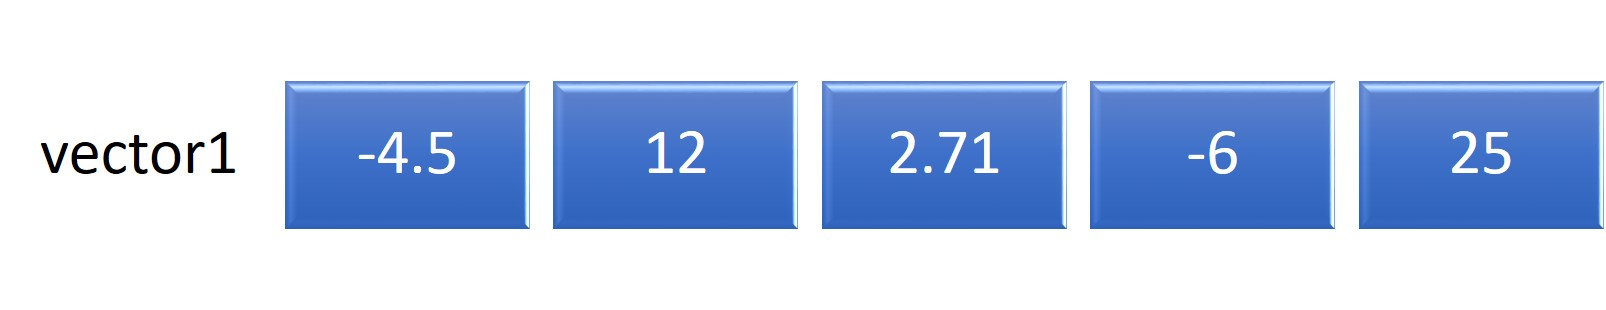
\includegraphics[width=0.8\linewidth]{images/10_vector1} 

}

\caption{Ejemplo vector numérico}\label{fig:vector1}
\end{figure}

Un ejemplo de un vector de tipo caracter llamado \emph{vector2} con 4 elementos puede ser:

\begin{figure}

{\centering 
\includegraphics[width=0.8\linewidth]{images/11_vector2} 

}

\caption{Ejemplo vector caracter}\label{fig:vector2}
\end{figure}

Los elementos en cada uno de estos vectores ocupan una determinada posición y pueden ser accedidos a través del uso de \textbf{índices}, expresados con corchetes al lado del nombre del vector. Por ejemplo, la acción \texttt{ESCRIBIR\ vector1{[}3{]}} nos mostrará el valor 2.71.

\begin{figure}

{\centering 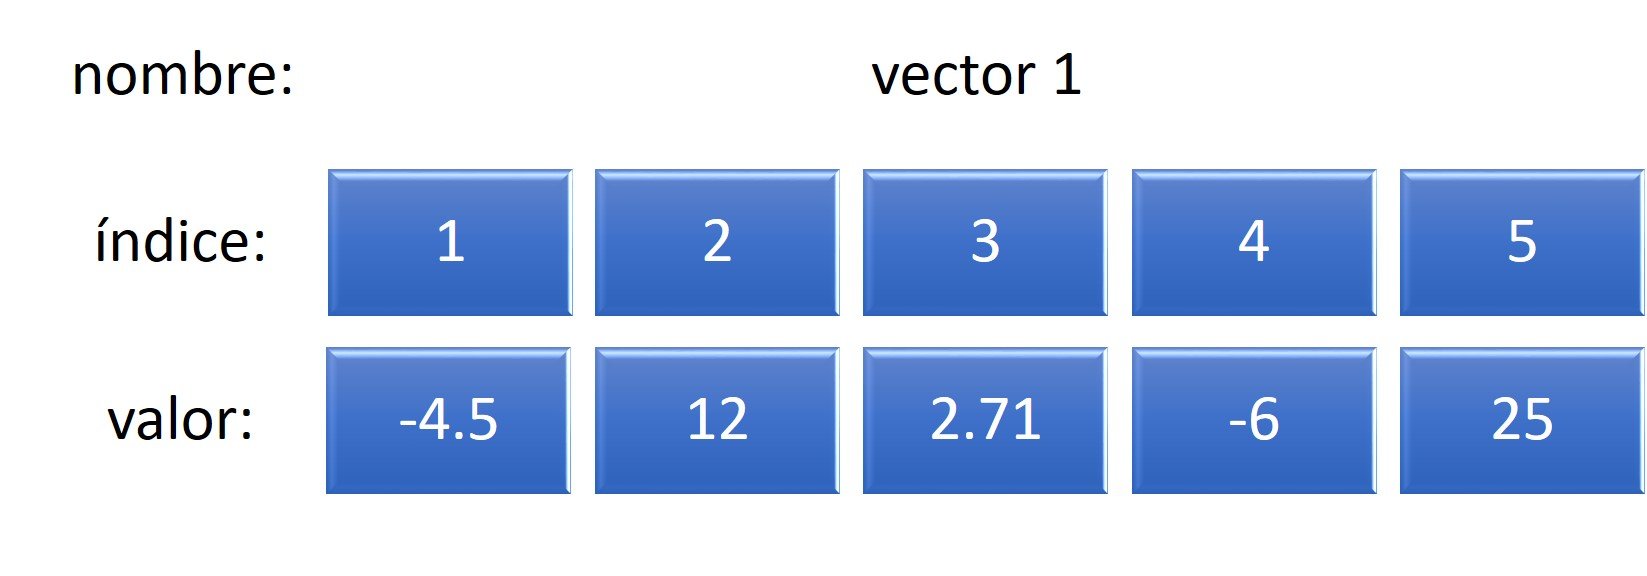
\includegraphics[width=0.8\linewidth]{images/12_vector1} 

}

\caption{Ejemplo vector numérico con posiciones indexadas}\label{fig:vector1bis}
\end{figure}

Como todas las variables que empleamos en nuestros algoritmos, los vectores deben ser declarados en el mismo y su tamaño debe ser especificado al comenzar. Esto se realiza a través de la acción \texttt{DIMENSIONAR}. Por ejemplo, el \emph{vector1} visto anteriomente puede ser creado de la siguiente forma:

\begin{Shaded}
\begin{Highlighting}[]
\NormalTok{DIMENSIONAR numérico vector1(5)}
\NormalTok{vector1[1] \textless{}{-} {-}4.5}
\NormalTok{vector1[2] \textless{}{-} 12}
\NormalTok{vector1[3] \textless{}{-} 2.71}
\NormalTok{vector1[4] \textless{}{-} {-}6}
\NormalTok{vector1[5] \textless{}{-} 25}
\end{Highlighting}
\end{Shaded}

Cuando declaramos un vector que usaremos más adelante, especificamos cuántos elementos entrarán en él poniendo su dimensión entre paréntesis al lado del nombre.

Podemos asignar valores a las posiciones del vector empleando estructuras de control iterativas, por ejemplo:

\begin{Shaded}
\begin{Highlighting}[]
\NormalTok{DIMENSIONAR numérico vector3(30)}
\NormalTok{PARA i DESDE 1 HASTA 30 HACER}
\NormalTok{    vector3[i] \textless{}{-} i * 2}
\NormalTok{FIN PARA}
\end{Highlighting}
\end{Shaded}

En este ejemplo, la variable \texttt{i} se usa como índice para el espacio en el vector que será modificado y también para calcular el valor por asignar, resultando en un vector con los números 2, 4, 6, \ldots, 60.

En el próximo ejemplo, se deja que el usuario determine la dimensión del vector y que provea cada uno de los valores para el mismo:

\begin{Shaded}
\begin{Highlighting}[]
\NormalTok{VARIABLE numérico tam}
\NormalTok{LEER tam}
\NormalTok{DIMENSIONAR numérico vector4(tam)}
\NormalTok{PARA i DESDE 1 HASTA tam HACER}
\NormalTok{    LEER vector4[i]}
\NormalTok{FIN PARA}
\end{Highlighting}
\end{Shaded}

\hypertarget{arreglos-bidimensionales}{%
\section{Arreglos bidimensionales}\label{arreglos-bidimensionales}}

Un \textbf{arreglo bidimensional} representa lo que habitualmente conocemos con una \textbf{matriz} y también lo podemos llamar de esa forma. A diferencia de los vectores, las matrices requieren dos índices o parámetros para acceder a sus elementos, sobre los cuales nos referimos como \textbf{fila} y \textbf{columna}. Se pueden utilizar dos estructuras \emph{PARA\ldots{} FIN PARA} anidadas para recorrer todos los elementos de la matriz, como se muestra en el siguiente ejemplo:

\begin{Shaded}
\begin{Highlighting}[]
\NormalTok{DIMENSIONAR numérico matriz1(3, 4)}
\NormalTok{PARA i DESDE 1 HASTA 3 HACER}
\NormalTok{    PARA j DESDE 1 HASTA 4 HACER}
\NormalTok{        matriz1[i, j] \textless{}{-} i * j}
\NormalTok{    FIN PARA}
\NormalTok{FIN PARA}
\end{Highlighting}
\end{Shaded}

\begin{figure}

{\centering 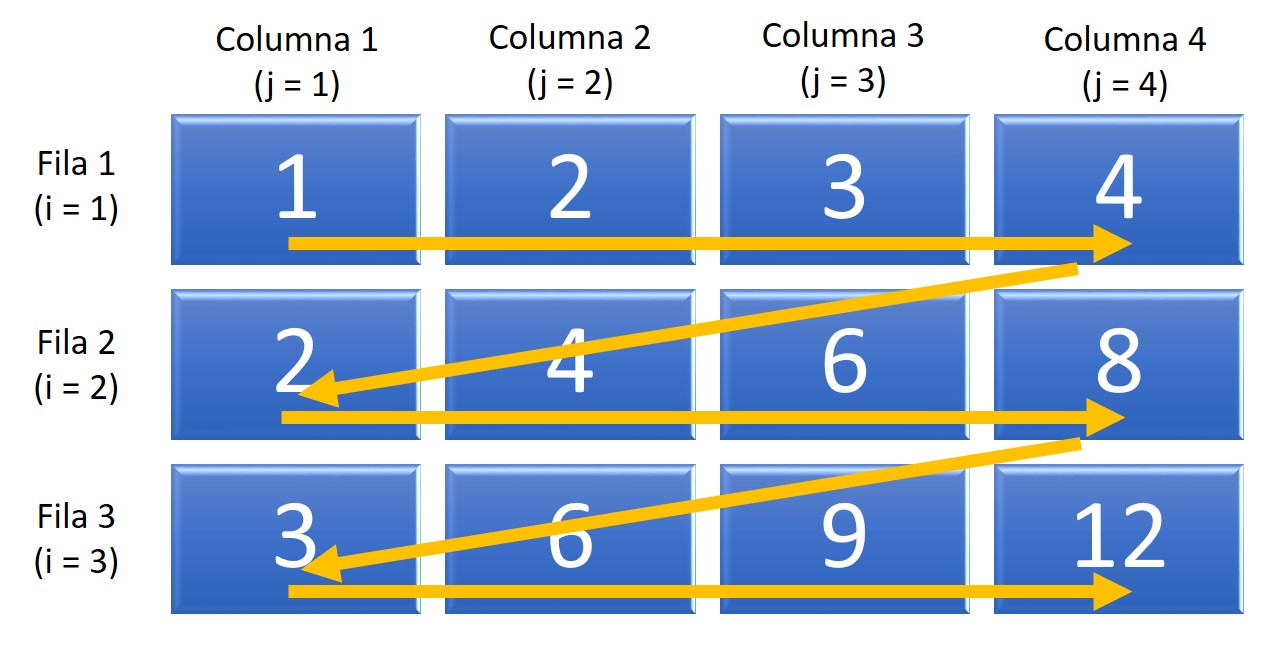
\includegraphics[width=0.8\linewidth]{images/13_matriz1} 

}

\caption{Ejemplo: matriz1}\label{fig:matriz1}
\end{figure}

En el ejemplo anterior los valores fueron asignados recorriendo la matriz por filas como lo indican las flechas. Otra posibilidad es recorrer la matriz por columna en primer instancia, para lo cual la estructura \emph{PARA\ldots{} FIN PARA} que representa a los índices de las columnas debe ser la externa y la que representa a los índices de columnas, la interna:

\begin{Shaded}
\begin{Highlighting}[]
\NormalTok{DIMENSIONAR numérico matriz1(3, 4)}
\NormalTok{PARA j DESDE 1 HASTA 4 HACER}
\NormalTok{    PARA i DESDE 1 HASTA 3 HACER}
\NormalTok{        matriz1[i, j] \textless{}{-} i * j}
\NormalTok{    FIN PARA}
\NormalTok{FIN PARA}
\end{Highlighting}
\end{Shaded}

\begin{figure}

{\centering 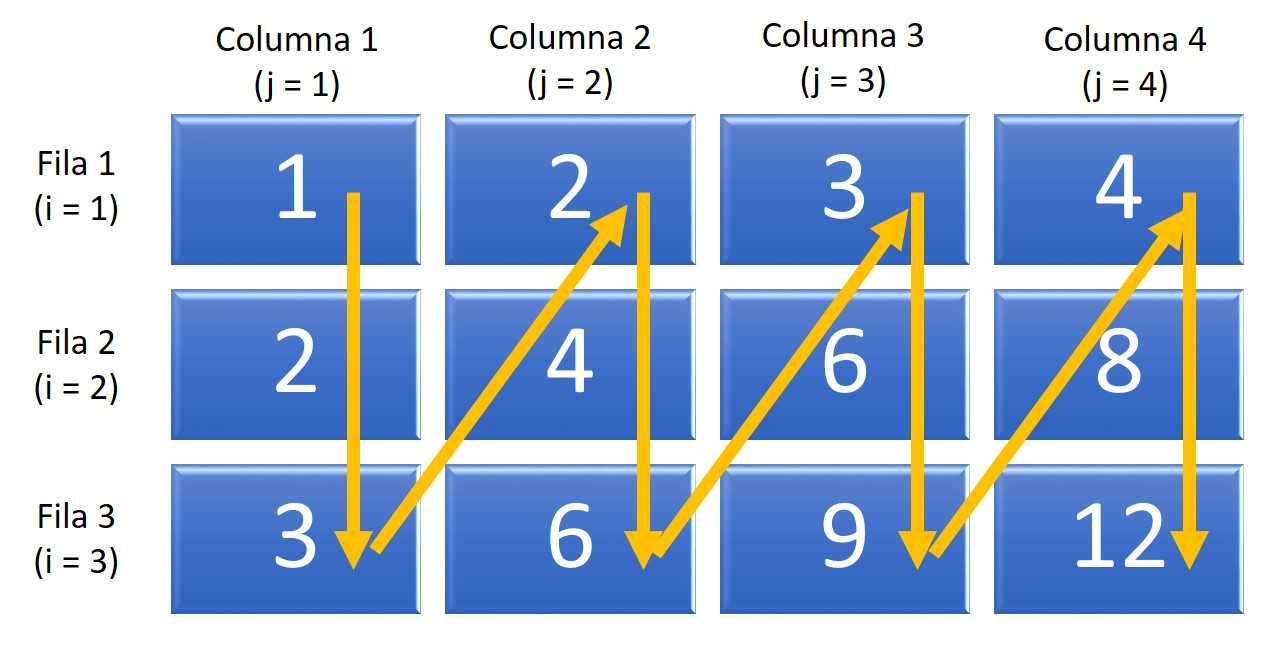
\includegraphics[width=0.8\linewidth]{images/13_matriz1bis} 

}

\caption{Ejemplo: matriz1 recorrida por columnas}\label{fig:matriz1bis}
\end{figure}

\hypertarget{arreglos-multidimensionales}{%
\section{Arreglos multidimensionales}\label{arreglos-multidimensionales}}

Un \textbf{arreglo multidimensional} contiene más de dos dimensiones. Aunque los vectores y matrices son los tipos de arreglos más usados, podemos emplear tantos índices para localizar los elementos del arreglo como estimemos necesarios. La representación matemática o visual ya no es tan sencilla. Para interpretarlos o saber cuándo usarlos, pensamos que cada uno de las dimensiones representa una característica, condicionante o parámetro definidor del elemento.

Por ejemplo, si se desea contar el número de autos que ingresaron a una playa de estacionamiento por hora a lo largo de varios años, podríamos utilizar un arreglo donde la primera dimensión indique el año, la segunda el mes, la tercera el día y la cuarta la hora. Si llamamos a este arreglo \texttt{numeroAutos}, el elemento \texttt{numeroAutos{[}2,\ 4,\ 23,\ 14{]}} contendrá el número de autos que ingresaron a la hora 14, del día 23, en el mes 4 del segundo año.

\hypertarget{ejemplo-invertir-los-elementos-de-un-vector}{%
\section{Ejemplo: invertir los elementos de un vector}\label{ejemplo-invertir-los-elementos-de-un-vector}}

Nos planteamos el problema de dar vuelta los elementos pertenecientes a un vector, de manera que el primer elemento pase a ser el último, el segundo pase al penúltimo lugar, etcétera.

Por ejemplo, dado el vector \texttt{v}:

\begin{figure}

{\centering 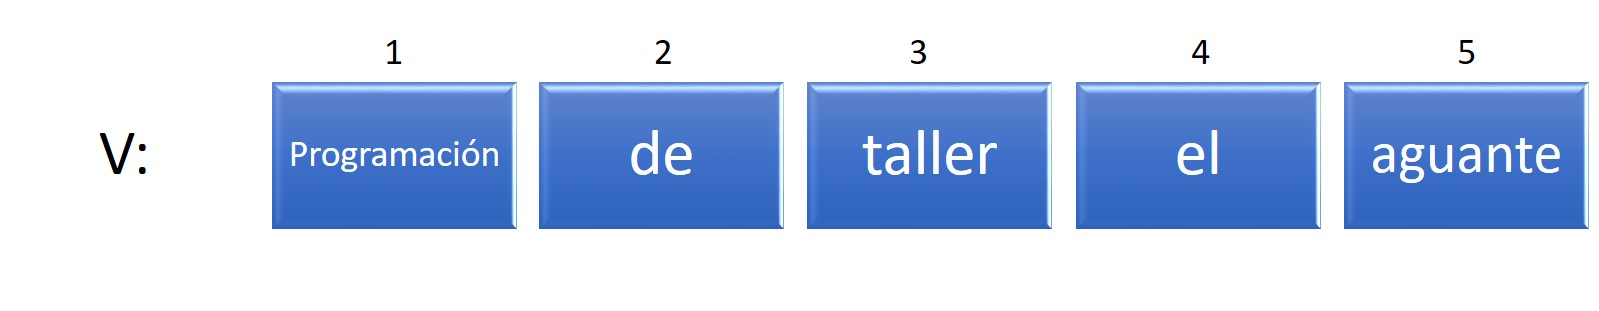
\includegraphics[width=0.8\linewidth]{images/14_invertir1} 

}

\caption{Vector v original}\label{fig:inv1}
\end{figure}

Queremos modificarlo para obtener:

\begin{figure}

{\centering 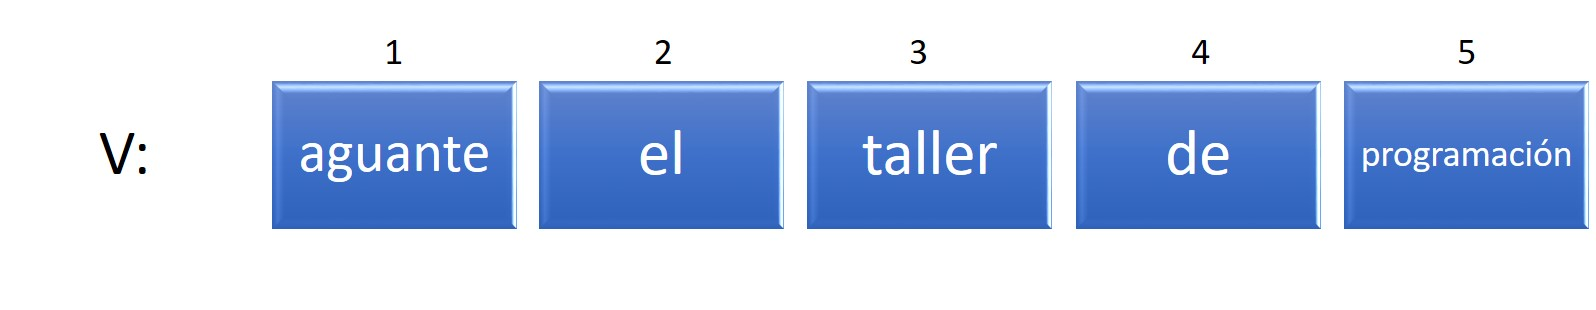
\includegraphics[width=0.8\linewidth]{images/15_invertir1} 

}

\caption{Vector v reordenado}\label{fig:inv2}
\end{figure}

Si bien podemos pensar en distintas formas para resolver este problema, probablemente la más sencilla requiere que intercambiemos de a dos los valores en ciertas posiciones del vector, por ejemplo, el primero y el último. Para esto podemos emplear una variable auxiliar para guardar el valor de alguna de las celdas temporariamente (por eso lo vamos a llamar \texttt{tmp}) y poder realizar el intercambio:

\begin{figure}

{\centering 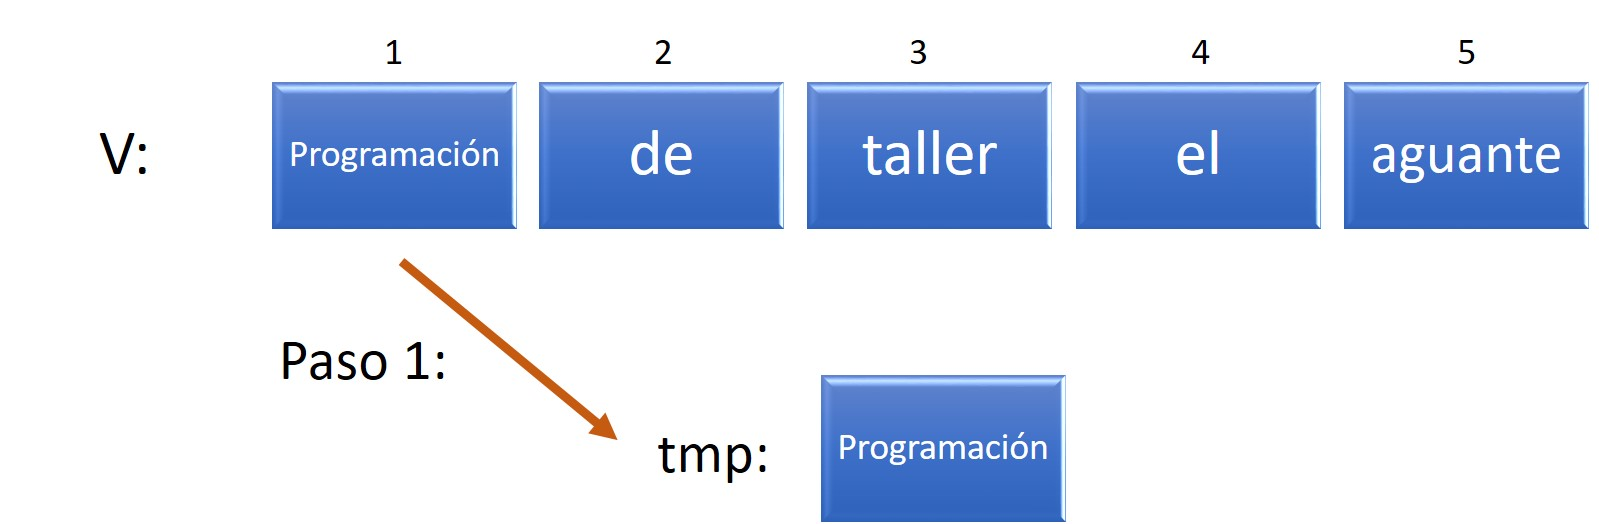
\includegraphics[width=0.8\linewidth]{images/16_invertir} 

}

\caption{Vector v reordenado}\label{fig:inv3}
\end{figure}

\begin{figure}

{\centering 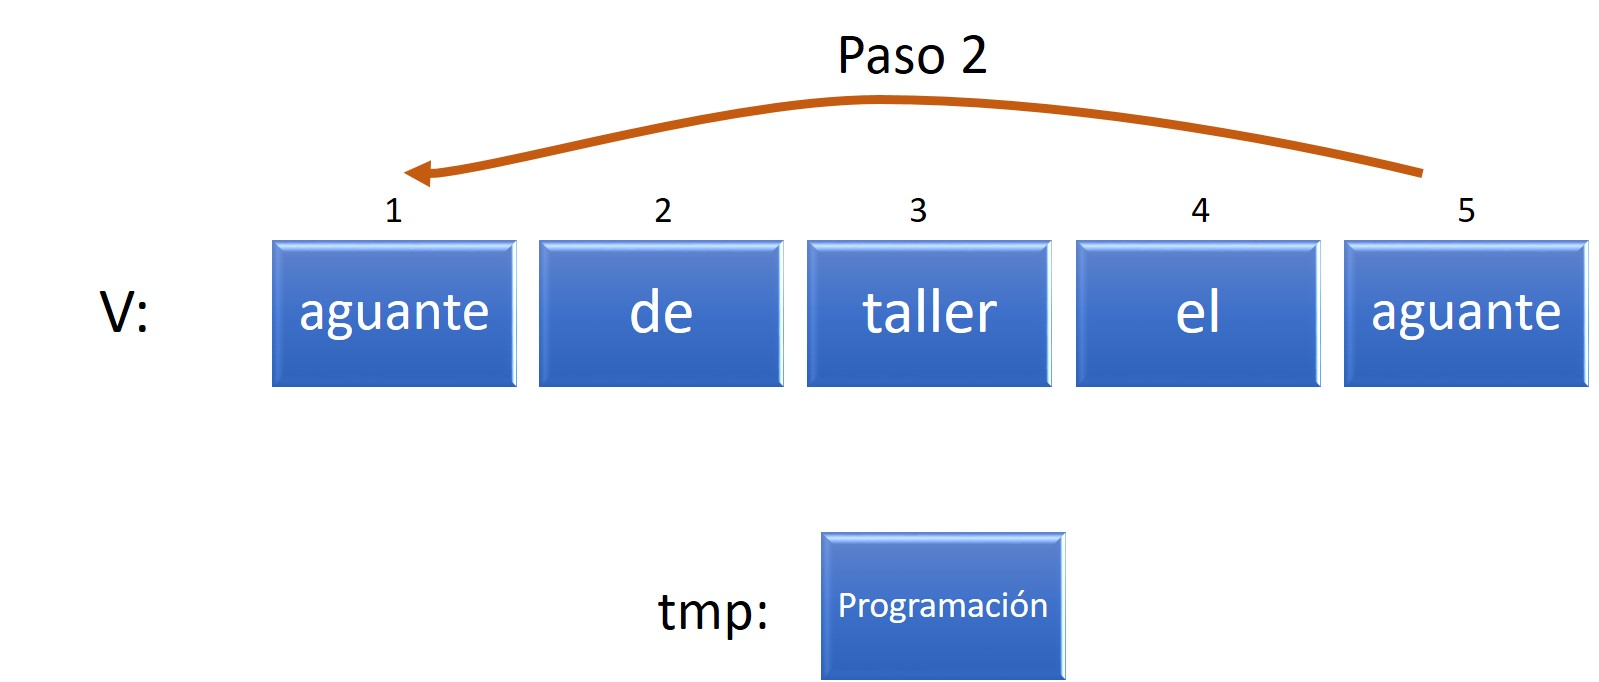
\includegraphics[width=0.8\linewidth]{images/17_invertir} 

}

\caption{Vector v reordenado}\label{fig:inv4}
\end{figure}

\begin{figure}

{\centering 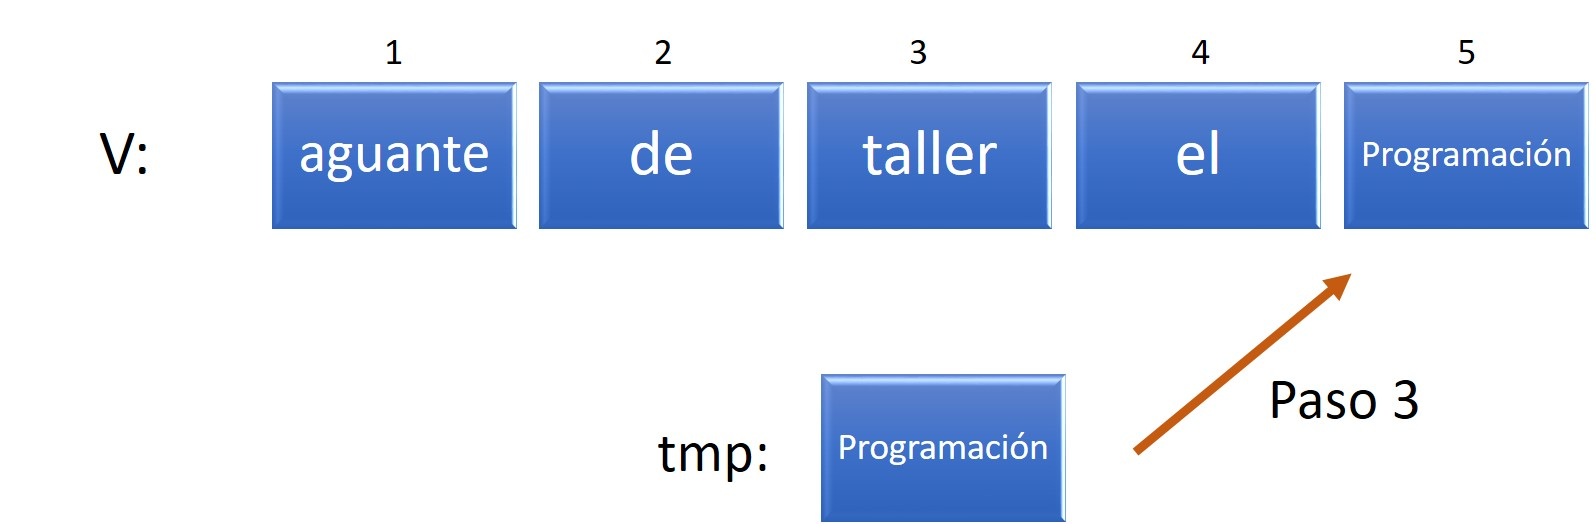
\includegraphics[width=0.8\linewidth]{images/18_invertir} 

}

\caption{Vector v reordenado}\label{fig:inv5}
\end{figure}

Ahora sólo resta realizar el mismo procedimiento para los valores de las posiciones 2 y 4. Como el número de elementos en el vector es impar, el valor en la posición central queda en su lugar. Podemos definir el siguiente algorimo para resolver este problema de manera general:

\begin{Shaded}
\begin{Highlighting}[]
\NormalTok{ALGORITMO: "Invertir (dar vuelta) los elementos de un vector"}
\NormalTok{COMENZAR}
    
\NormalTok{    \textbackslash{}\textbackslash{} Declarar variables}
\NormalTok{    VARIABLE numérico n}
\NormalTok{    VARIABLE caracter tmp}
\NormalTok{    LEER n}
\NormalTok{    DIMENSIONAR caracter v(n)}
    
\NormalTok{    \textbackslash{}\textbackslash{} Asignar valores al vector}
\NormalTok{    PARA i DESDE 1 HASTA n HACER}
\NormalTok{        LEER v[i]}
\NormalTok{    FIN PARA}
    
\NormalTok{    \textbackslash{}\textbackslash{} Reordenar}
\NormalTok{    PARA i DESDE 1 HASTA ENTERO(n / 2) HACER}
\NormalTok{        tmp \textless{}{-} v[i]                 \textbackslash{}\textbackslash{} Paso 1}
\NormalTok{        v[i] \textless{}{-} v[n {-} i + 1]        \textbackslash{}\textbackslash{} Paso 2}
\NormalTok{        v[n {-} i + 1] \textless{}{-} tmp         \textbackslash{}\textbackslash{} Paso 3}
\NormalTok{    FIN PARA}
    
\NormalTok{    \textbackslash{}\textbackslash{} Mostrar el vector reodenado}
\NormalTok{    PARA i DESDE 1 HASTA n HACER}
\NormalTok{        ESCRIBIR v[i]}
\NormalTok{    FIN PARA}
    
\NormalTok{FIN}
\end{Highlighting}
\end{Shaded}

El código correspondiente en SAS/IML es:

\begin{Shaded}
\begin{Highlighting}[]
\NormalTok{/* Invertir (dar vuelta) un vector */}
\NormalTok{proc iml;}
\NormalTok{    v = \{"programacion" "de" "taller" "el" "aguante"\};}
\NormalTok{    n = ncol(v);}
\NormalTok{    do i = 1 to int(n / 2);}
\NormalTok{        tmp = v[i];}
\NormalTok{        v[i] = v[n {-} i + 1];}
\NormalTok{        v[n {-} i + 1] = tmp;}
\NormalTok{    end;}
\NormalTok{    print v;}
\NormalTok{quit;}
\end{Highlighting}
\end{Shaded}

\hypertarget{archivos}{%
\chapter{Archivos}\label{archivos}}

Como hemos visto, los programas usan variables para guardar información: datos de entrada, resultados calculados, valores intermedios. Sin embargo, la información guardada en las variables es efímera. Cuando los programas paran de correr, el valor almacenado en las variables se pierde. En muchas ocasiones, es necesario guardar información de una forma más permanente.

En estos casos, el enfoque usual es recolectar la información en un todo lógicamente cohesivo y guardarlo en un medio permanente que generalmente se graba en el disco rígido de la máquina, es decir, en un archivo. Un \textbf{archivo} o \textbf{fichero} es un conjunto de información sobre un mismo tema tratado como una unidad de almacenamiento y organizado de forma estructurada para la búsqueda de un dato individual. Los archivos pueden contener instrucciones de programas o información creada o usada por un programa. Todos los objetos de datos permanentes que guardamos en nuestra computadora (documentos, juegos, programas ejecutables, código, etc.) son guardados en la forma de archivos.

La unidad elemental que compone a un archivo o fichero es un \textbf{registro}, el cual es una colección de información relativa a una misma entidad. En general, cada registro de un mismo archivo tiene la misma estructura que los demás. Los datos individuales sobre dicha entidad ocupan \textbf{campos} dentro de los registros. Por ejemplo:

\begin{Shaded}
\begin{Highlighting}[]
\NormalTok{ARCHIVO: Pasajeros}
\NormalTok{Campo 1: NOMBRE, tipo caracter}
\NormalTok{Campo 2: NÚMERO DE VUELO, tipo caracter}
\NormalTok{Campo 3: FECHA DE VUELO, tipo caracter}
\NormalTok{Campo 4: NÚMERO DE ASIENTO, tipo caracter}
\NormalTok{Campo 5: CIUDAD ORIGEN, tipo caracter}
\NormalTok{Campo 6: CIUDAD DESTINO, tipo caracter}
\NormalTok{Campo 7: PRECIO, tipo numérico}
\end{Highlighting}
\end{Shaded}

\begin{longtable}[]{@{}
  >{\centering\arraybackslash}p{(\columnwidth - 12\tabcolsep) * \real{0.2048}}
  >{\centering\arraybackslash}p{(\columnwidth - 12\tabcolsep) * \real{0.1205}}
  >{\centering\arraybackslash}p{(\columnwidth - 12\tabcolsep) * \real{0.1446}}
  >{\centering\arraybackslash}p{(\columnwidth - 12\tabcolsep) * \real{0.1446}}
  >{\centering\arraybackslash}p{(\columnwidth - 12\tabcolsep) * \real{0.1084}}
  >{\raggedright\arraybackslash}p{(\columnwidth - 12\tabcolsep) * \real{0.1687}}
  >{\raggedright\arraybackslash}p{(\columnwidth - 12\tabcolsep) * \real{0.1084}}@{}}
\toprule()
\begin{minipage}[b]{\linewidth}\centering
Nombre
\end{minipage} & \begin{minipage}[b]{\linewidth}\centering
NroVuelo
\end{minipage} & \begin{minipage}[b]{\linewidth}\centering
FechaVuelo
\end{minipage} & \begin{minipage}[b]{\linewidth}\centering
NroAsiento
\end{minipage} & \begin{minipage}[b]{\linewidth}\centering
Origen
\end{minipage} & \begin{minipage}[b]{\linewidth}\raggedright
Destino
\end{minipage} & \begin{minipage}[b]{\linewidth}\raggedright
Precio
\end{minipage} \\
\midrule()
\endhead
Pamela Suárez & AR6071 & 12/09/17 & 17A & Rosario & Córdoba & 1532.23 \\
Gonzalo Echarri & AR5423 & 14/09/17 & 31B & Rosario & Buenos Aires & 1424.10 \\
\ldots{} & \ldots{} & \ldots{} & \ldots{} & \ldots{} & \ldots{} & \ldots{} \\
\bottomrule()
\end{longtable}

La forma más común de identificar un registro es eligiendo un campo dentro del registro llamado \textbf{clave} (por ejemplo, el nombre del pasajero), que contiene un único valor para cada registro. En otras casos es posible identificar un registro a través del valor de más de uno de sus campos.

\hypertarget{organizaciuxf3n-de-archivos}{%
\section{Organización de archivos}\label{organizaciuxf3n-de-archivos}}

Existen distintos tipos de organización de los archivos según la forma en la que se pueda acceder a cada uno de sus registros:

\begin{itemize}
\item
  Archivo secuencial

  Los registros se encuentran en cierto orden que debe ser respetado para la lectura de los mismos. Para leer el registro situado en la posición \emph{n}, el programa previamente tiene que pasar por todos los registros que ocupan las posiciones anteriores. Los registros pueden leerse uno por uno hasta llegar al final del archivo. La mayoría de los lenguajes de programación disponen de una función lógica que devuelve un valor \textbf{VERDADERO} cuando se alcanza el final del archivo.
\item
  Archivo directo

  Está formado por un conjunto de registros que pueden ser recuperados por su posición dentro del archivo sin necesidad de recorrer los anteriores.
\item
  Archivo indexado

  Dispone de una tabla de índices adicional, es decir, una referencia que permite obtener de forma automática la ubicación de la zona del archivo donde se encuentra el registro buscado. Esto permite localizar un registro por medio de su clave, o del valor de algún campo en particular, sin recorrer previamente los registros que lo preceden.
\end{itemize}

La organización más sencilla y más comunmnete empleada es la secuencial, aunque no sea la más eficiente. Nosotros trabajaremos en el Taller con este tipo de organización.

\hypertarget{operaciones-sobre-archivos}{%
\section{Operaciones sobre archivos}\label{operaciones-sobre-archivos}}

Los procedimientos básicos que los programas pueden llevar a cabo sobre los distintos tipos de archivos son:

\begin{itemize}
\item
  Creación de un archivo

  Consiste en la escritura de los registros que van a conformar el archivo. Los datos pueden introducirse por teclado, desde otro archivo o como resultado de algún proceso intermedio.
\item
  Apertura y cierre de un archivo

  Para que un programa pueda operar directamente sobre un archivo, la primera operación que debe realizar es la \textbf{apertura} del mismo, que incluye la identificación del archivo a utilizar y el modo (lectura, escritura, etc.). Cuando un programa no vaya a acceder más a un archivo, es necesario indicarlo a través del \textbf{cierre} del mismo, ya que se liberan memoria y recursos del sistema, se previene la corrupción de los datos si se detiene el programa mientras se está ejecutando y expresa explícitamente que ya no se hará más uso del mismo.
\item
  Lectura y escritura en un archivo

  La \textbf{lectura} consiste en transferir información del archivo a la memoria principal usada por el programa, mientras que la \textbf{escritura} es la transferencia de información guardada en las variables del programa al archivo.
\end{itemize}

Otras operaciones que se pueden realizar sobre los archivos incluyen acciones de:

\begin{itemize}
\tightlist
\item
  Actualización: añadir (dar de alta), modificar o eliminar (dar de baja) algún registro.
\item
  Clasificación: reubicar los registros de tal forma que queden ordenados por algún campo determinado.
\item
  Fusión o mezcla: combinar dos o más archivos para formar uno nuevo.
\item
  Partición: subdividir los registros por el valor que toman en algún campo.
\end{itemize}

\hypertarget{pseudo-cuxf3digo}{%
\section{Pseudo-código}\label{pseudo-cuxf3digo}}

Al escribir los algoritmos en pseudo-código, se puede hacer uso de las siguientes expresiones para representar algunas operaciones a realizar sobre los archivos:

\begin{itemize}
\tightlist
\item
  \texttt{ABRIR\ (nombre\ del\ archivo)\ secuencial,\ de\ entrada/salida}: indica la acción de apertura de un archivo con organización secuencial, sobre el cual se va a proceder a realizar lectura o escritura de registros.
\item
  \texttt{CERRAR\ (nombre\ del\ archivo)}: para indicar que el archivo no será vuelto a utilizar.
\item
  \texttt{LEER\ (nombre\ del\ archivo)\ campo1,\ campo2,\ ...}: indica la lectura del próximo registro cuando se trabaja con un archivo secuencial. La expresión \texttt{campo1,\ campo2,\ ...} son los nombres de los campos que contienen los registros y constituyen los identificadores de las variables que almacenarán temporalmente los datos del registro que se están leyendo.
\item
  \texttt{LEER\ (nombre\ del\ archivo,\ número\ de\ registro)\ campo1,\ campo2,\ ...}: indica la lectura de un registro en particular cuando se trabaja con un archivo de acceso directo.
\item
  \texttt{LEER\ (nombre\ del\ archivo,\ campo1\ =\ valor)\ campo1,\ campo2,\ ...}: indica la lectura de cada uno de los registros en los cuales el campo \texttt{campo1} es igual a \texttt{valor}, para cuando se trabaja con un archivo de acceso indexado.
\item
  Las tres acciones de \texttt{LEER} anteriores tienen su acción análoga de \texttt{ESCRIBIR}, para modificar o añadir registros al archivo.
\item
  \texttt{FINDE\ (nombre\ del\ archivo)}: es la función lógica que devuelve el valor \texttt{FALSO} mientras resten más registros por leer en el archivo y el valor \texttt{VERDADERO} cuando se llega al final del archivo y ya no quedan más registros por leer.
\end{itemize}

\hypertarget{ejemplo-lectura-de-un-archivo}{%
\subsection{Ejemplo: lectura de un archivo}\label{ejemplo-lectura-de-un-archivo}}

Siendo \texttt{nombreArchivo} el nombre del archivo que se desea leer, compuesto por \texttt{m} campos llamados \texttt{campo1}, \texttt{campo2}, \ldots, \texttt{campom}, entonces, el pseudocódigo necesario para leer el archivo es:

\begin{Shaded}
\begin{Highlighting}[]
\NormalTok{ABRIR(nombreArchivo) secuencial, de entrada}
\NormalTok{MIENTRAS FINDE(nombreArchivo) = FALSO ENTONCES}
\NormalTok{    LEER(nombreArchivo) campo1, campo2, ..., campom}
    
\NormalTok{    ... realizar operaciones con las variables campo1, campo2, ..., campom...}
    
\NormalTok{FIN MIENTRAS}
\NormalTok{CERRAR(nombreArchivo)}
\end{Highlighting}
\end{Shaded}

En IML, podemos seguir los siguientes pasos:

\begin{enumerate}
\def\labelenumi{\arabic{enumi}.}
\tightlist
\item
  Haciendo uso de un \texttt{proc\ import}, se importa el archivo en la librería temporal \texttt{Work} (podría guardarse en otra), creando un dataset cuyo nombre se indica en \texttt{out} (en este caso, \texttt{nombreDataset}):
\end{enumerate}

\begin{Shaded}
\begin{Highlighting}[]
\NormalTok{* Si se trata de un archivo de texto;}
\NormalTok{proc import out = nombreDataset}
\NormalTok{            datafile = "C:\textbackslash{}direccion\textbackslash{}hasta\textbackslash{}la\textbackslash{}carpeta\textbackslash{}nombreArchivo.txt"}
\NormalTok{            dbms = TAB REPLACE;}
\NormalTok{run;}
            
\NormalTok{* Si se trata de un archivo de Excel;}
\NormalTok{proc import out = nombreDataset}
\NormalTok{            datafile = "C:\textbackslash{}direccion\textbackslash{}hasta\textbackslash{}la\textbackslash{}carpeta\textbackslash{}nombreArchivo.txt"}
\NormalTok{            dbms = EXCEL REPLACE;}
\NormalTok{run;}
\end{Highlighting}
\end{Shaded}

\begin{enumerate}
\def\labelenumi{\arabic{enumi}.}
\setcounter{enumi}{1}
\tightlist
\item
  Dentro del \texttt{proc\ iml}, leer línea por línea los registros del data set que hemos creado (en este ejemplo, \texttt{nombreDataset}) a través de un \texttt{do\ data;}:
\end{enumerate}

\begin{Shaded}
\begin{Highlighting}[]
\NormalTok{proc iml;}

\NormalTok{    ...}

\NormalTok{    use nombreDataset;}
\NormalTok{    do data;}
    
\NormalTok{        * Se lee de a una línea (registro) por vez, los campos del archivo son usados como}
\NormalTok{            variables que tienen los respectivos valores para la línea en cuestión;}
        
\NormalTok{       ... realizar operaciones con los valores de cada registro del archivo...}
            
\NormalTok{    end;}
\NormalTok{    close nombreDataset;}

\NormalTok{    ...}

\NormalTok{quit;}
\end{Highlighting}
\end{Shaded}

\hypertarget{ejemplo-escritura-de-un-archivo}{%
\subsection{Ejemplo: escritura de un archivo}\label{ejemplo-escritura-de-un-archivo}}

Supongamos que la información que se desea guardar en un nuevo archivo se encuentra en una matriz llamada \texttt{tabla}, que tiene \texttt{n} filas correspondientes a \texttt{n} registros y \texttt{m} columnas referidos a \texttt{m} campos llamados \texttt{campo1}, \texttt{campo2}, \ldots, \texttt{campom}. Entonces, el pseudocódigo necesario para crear y escribir el nuevo archivo es:

\begin{Shaded}
\begin{Highlighting}[]
\NormalTok{CREAR(nombreArchivo)}
\NormalTok{ABRIR(nombreArchivo) secuencial, de salida}
\NormalTok{PARA i DESDE 1 HASTA n HACER}
\NormalTok{    campo1 \textless{}{-} tabla[i, 1]}
\NormalTok{    campo2 \textless{}{-} tabla[i, 2]}
\NormalTok{    ...}
\NormalTok{    campom \textless{}{-} tabla[i, m]}
\NormalTok{    ESCRIBIR(nombreArchivo) campo1, campo2, ..., campom}
\NormalTok{FIN PARA}
\NormalTok{CERRRAR(nombreArchivo)}
\end{Highlighting}
\end{Shaded}

En IML, a partir de la matriz que tiene la información que se desea guardar en un archivo, se deben seguir dos pasos:

\begin{enumerate}
\def\labelenumi{\arabic{enumi}.}
\tightlist
\item
  Dentro del mismo \texttt{proc\ iml}, crear un dataset de SAS a partir de la matriz. En este ejemplo, la matriz se llama \texttt{tabla}, el nuevo dataset \texttt{datos} y se guarda en la librería temporal \texttt{Work} (podría guardarse en otra):
\end{enumerate}

\begin{Shaded}
\begin{Highlighting}[]
\NormalTok{proc iml;}
    
\NormalTok{    ... todo el código necesario ...}

\NormalTok{    create datos from tabla[colname = ("campo1" || "campo2" || ... || "campom")];}
\NormalTok{    append from tabla;}
\NormalTok{    close datos;}
\NormalTok{quit;}
\end{Highlighting}
\end{Shaded}

\begin{enumerate}
\def\labelenumi{\arabic{enumi}.}
\setcounter{enumi}{1}
\tightlist
\item
  Haciendo uso de un \texttt{proc\ export}, se exporta el dataset desde la librería Work hasta una carpeta de la computadora, en este ejemplo, como archivo de texto:
\end{enumerate}

\begin{Shaded}
\begin{Highlighting}[]
\NormalTok{proc export data = datos}
\NormalTok{            outfile = "C:\textbackslash{}direccion\textbackslash{}hasta\textbackslash{}la\textbackslash{}carpeta\textbackslash{}deseada\textbackslash{}nombreArchivo.txt" }
\NormalTok{            dbms = TAB REPLACE;}
\NormalTok{run;}
\end{Highlighting}
\end{Shaded}

\hypertarget{archivos-de-texto}{%
\section{Archivos de texto}\label{archivos-de-texto}}

Archivos como el del ejemplo de los pasajeros suelen ser guardados como \textbf{archivos de texto}. Un \textbf{archivo de texto} (también conocido como \emph{texto llano} o \emph{texto simple}), es un archivo informático que contiene únicamente texto formado por una secuencia ordenada de caracteres. El texto almacenado en este tipo de archivo carece de cualquier tipo de formato tipográfico (negrita, cursiva, colores, subrayado, fuente, etc.), lo cual permite que una gran variedad de programas pueda leer y editar el contenido.

Los archivos de texto están compuestos por caracteres ordinarios, como las letras, números y signos de puntuación, y por caracteres especiales que indican, por ejemplo, saltos de línea y tabulaciones. Como las computadoras solamente entienden números, cada caracter es codificado internamente con un representación numérica binaria. Distinas maneras de hacer esta representación dan lugar a diferentes formatos de codificación de caracteres (como \emph{ASCII}, \emph{ISO-8859-1} o \emph{UTF-8}).

La información contenida en los archivos que utilizaremos en el Taller puede ser almacenada de manera práctica en archivos de texto.

\hypertarget{subalgortimos}{%
\chapter{Subalgortimos}\label{subalgortimos}}

Un principio fundamental en la resolución de un problema es intentar descomponerlo en partes más pequeñas, que puedan ser más fáciles de afrontar. Este concepto también se aplica en la programación. Nuestros algoritmos pueden descomponerse en \textbf{subalgoritmos} que den solución a un aspecto del problema, de menor extensión. Este proceso se conoce como \textbf{descomposición algorítmica} o \textbf{descomposición modular}. Cada subalgoritmo debe ser independiente de los demás y a su vez podría seguir descomponiéndose en partes más sencillas en lo que se conoce como \textbf{refinamiento sucesivo}. Si un programa es muy largo se corre el riesgo de que sea muy difícil de entender como un todo, pero siempre se lo puede dividir en secciones más simples y manejables. Un subalgoritmo se escribe una vez y luego es utilizado por todos aquellos algoritmos que lo necesiten.

Observemos el siguiente ejemplo, que presenta un algoritmo para el cálculo de un número combinatorio. Recordemos que el número combinatorio entre \(n\) y \(k\) se define como:

\[ {n \choose k} = \frac{n!}{(n-k)!k!} \hspace{1cm} k \le n, k \in \mathbb{N}_0, n \in \mathbb{N}\]

\begin{Shaded}
\begin{Highlighting}[]
\NormalTok{ALGORITMO: Ej 1. Cálculo de números combinatorios}
\NormalTok{COMENZAR}
\NormalTok{    VARIABLE numerica n, k, fact1, fact2, fact3, comb}
\NormalTok{    LEER n, k \textbackslash{}\textbackslash{} Asumimos que n y k cumplen con los requisitos}

\NormalTok{    \textbackslash{}\textbackslash{} Calcular el factorial de n}
\NormalTok{    fact1 \textless{}{-} 1}
\NormalTok{    PARA i DESDE 1 HASTA n HACER}
\NormalTok{        fact1 \textless{}{-} fact1 * i}
\NormalTok{    FIN PARA}

\NormalTok{    \textbackslash{}\textbackslash{} Calcular el factorial de n{-}k}
\NormalTok{    fact2 \textless{}{-} 1}
\NormalTok{    PARA i DESDE 1 HASTA n {-} k HACER}
\NormalTok{        fact2 \textless{}{-} fact2 * i}
\NormalTok{    FIN PARA}

\NormalTok{    \textbackslash{}\textbackslash{} Calcular el factorial de k}
\NormalTok{    fact3 \textless{}{-} 1}
\NormalTok{    PARA i DESDE 1 HASTA k HACER}
\NormalTok{        fact3 \textless{}{-} fact3 * i}
\NormalTok{    FIN PARA}

\NormalTok{    \textbackslash{}\textbackslash{} Calcular el nro combinatorio}
\NormalTok{    comb \textless{}{-} fact1 / (fact2 * fact3)}

\NormalTok{    ESCRIBIR "El nro combinatorio de " n " tomado de a " k " es " comb}
\NormalTok{FIN}
\end{Highlighting}
\end{Shaded}

Como se puede observar, el cálculo del factorial requiere siempre la misma estructura y se repite tres veces. Esto constituye una parte del problema cuya resolución puede plantearse por separado, dando lugar a un subalgoritmo. El algoritmo quedaría mejor expresado de la siguiente manera:

\begin{Shaded}
\begin{Highlighting}[]
\NormalTok{ALGORITMO: Ej 2. Cálculo de números combinatorios}
\NormalTok{COMENZAR}
\NormalTok{    VARIABLE numérica n, k, comb}
\NormalTok{    LEER n, k }
\NormalTok{    comb \textless{}{-} factorial(n) / (factorial(n {-} k) * factorial(k))}
\NormalTok{    ESCRIBIR "El nro combinatorio de " n " tomado de a " k " es " comb}
\NormalTok{FIN}
\end{Highlighting}
\end{Shaded}

Aquí se puede ver cómo se simplificó la estructura del algoritmo, al hacer uso de un subalgoritmo llamado \texttt{factorial} que toma entre paréntesis un valor para el que procede a calcular y devolver el factorial. Para que esto funcione, debemos definir aparte dicho subalgoritmo, como se muestra a continuación. Más adelante veremos los detalles de esta definición y por qué, en particular, se dice que este subalgoritmo es una \emph{función}:

\begin{Shaded}
\begin{Highlighting}[]
\NormalTok{FUNCIÓN factorial(n: numérico): numérico}
\NormalTok{    VARIABLE numérica fact}
\NormalTok{    fact \textless{}{-} 1}
\NormalTok{    PARA i DESDE 1 HASTA n HACER}
\NormalTok{        fact \textless{}{-} fact * i}
\NormalTok{    FIN PARA}
\NormalTok{    DEVOLVER fact}
\NormalTok{FIN FUNCIÓN}
\end{Highlighting}
\end{Shaded}

El empleo de subalgoritmos, desarrollando por separado ciertas partes del problema, resulta especialmente ventajoso en los casos siguientes:

\begin{itemize}
\tightlist
\item
  \textbf{En algoritmos complejos}: si el algoritmo, y luego el programa, se escribe todo seguido resulta muy complicado de entender, porque se pierde la visión de su estructura global dada la gran cantidad de operaciones que lo conforman. Aislando ciertas partes como subalgoritmos separados se reduce la complejidad.
\item
  \textbf{Cuando se repiten operaciones análogas}: si la resolución de un problema requiere realizar una tarea que se repite varias veces en el algoritmo, podemos definir dicha tarea como un subalgoritmo por separado. De esta manera, su código se escribirá sólo una vez aunque se use en muchos puntos del programa.
\end{itemize}

Los subalgoritmos se clasifican en \textbf{funciones} y \textbf{procedimientos}. Las \textbf{funciones} devuelven como resultado un solo valor al algoritmo principal. Los procedimientos, en cambio, pueden devolver cero, uno o varios valores.

\hypertarget{funciones}{%
\section{Funciones}\label{funciones}}

Una \textbf{función} es un subalgoritmo que devuelve un único resultado. Ya hemos trabajado con funciones que asumimos predefinidas, como por ejemplo las funciones módulo (\texttt{MOD}), valor absoluto (\texttt{ABS}) o raiz cuadrada (\texttt{RAIZ}), pero ahora veremos que podemos definir nuestras propias funciones. El valor que la función devuelve como resultado define su tipo, de modo que una función puede ser de tipo numérica, caracter o lógica. En programación, la noción de función se asemeja a la idea matemática de función de una o más variables. Por ejemplo, podemos pensar en la función \(f(x, y) = x^2 + 3y\). En pseudocódigo, el subalgoritmo que se encargaría de implementarla es:

\begin{Shaded}
\begin{Highlighting}[]
\NormalTok{FUNCIÓN f(x: numérico, y: numérico): numérico}
\NormalTok{COMENZAR}
\NormalTok{    DEVOLVER x ** 2 + 3 * y}
\NormalTok{FIN FUNCIÓN}
\end{Highlighting}
\end{Shaded}

Dado que esta función devuelve un valor numérico, decimos que la misma es de tipo numérico, lo cual se indica al final del encabezado. Se dice que \(x\) e \(y\) son los \textbf{parámetros formales} o \textbf{ficticios} y son los que permiten expresar la ``ley'' o ``forma'' de la función. También se aclara en el encabezado que estos parámetros son de tipo numérico. Los valores en los cuales se quiere evaluar la función se llaman \textbf{parámetros actuales} o \textbf{reales}. Por ejemplo, si nos interesa calcular \(f(4, 5)\), los valores \(4\) y \(5\) son los parámetros actuales y se establece una correspondencia entre el parámetro formal \(x\) y el real \(4\), así como entre la \(y\) y el \(5\). Como veremos más adelante, dicha correspondencia puede establecerse de distintas formas. En este ejemplo, el resultado que se obtiene es \(31\). A los parámetros también se les dice \textbf{argumentos}.

También puede ser expresada como:

\begin{Shaded}
\begin{Highlighting}[]
\NormalTok{FUNCIÓN f(x: numérico, y: numérico): numérico}
\NormalTok{COMENZAR}
\NormalTok{    VARIABLE numérica rtdo}
\NormalTok{    rtdo \textless{}{-} x ** 2 + 3 * y}
\NormalTok{    DEVOLVER rtdo}
\NormalTok{FIN FUNCIÓN}
\end{Highlighting}
\end{Shaded}

De manera general, la definición de una función es:

\begin{Shaded}
\begin{Highlighting}[]
\NormalTok{FUNCIÓN nombre(lista de parámetros formales): tipo de resultado}
\NormalTok{COMENZAR}
\NormalTok{    Declaración de variables}
\NormalTok{    Acciones}
\NormalTok{    DEVOLVER valor}
\NormalTok{FIN FUNCIÓN}
\end{Highlighting}
\end{Shaded}

La palabra clave \texttt{DEVOLVER} provoca la inmediata finalización de la ejecución de la función e indica cuál es el resultado de la misma, cuyo tipo debe coincidir con el tipo de función declarado antes. La acción \texttt{DEVOLVER} se puede insertar en cualquier punto de la parte ejecutable de la función y además es posible utilizar más de una sentencia \texttt{DEVOLVER} en una misma función, aunque sólo una llegue a ejecutarse. Esto puede verse en el siguiente ejemplo:

\begin{Shaded}
\begin{Highlighting}[]
\NormalTok{FUNCIÓN maximo(num1: numérico, num2: numérico): numérico}
\NormalTok{COMENZAR}
\NormalTok{    SI num1 \textgreater{}= num2}
\NormalTok{        ENTONCES}
\NormalTok{            DEVOLVER num1}
\NormalTok{        SI NO}
\NormalTok{            DEVOLVER num2}
\NormalTok{    FIN SI}
\NormalTok{FIN FUNCIÓN}
\end{Highlighting}
\end{Shaded}

Para usar una función en un algoritmo, se la invoca escribiendo su nombre seguida por los valores actuales entre paréntesis, separados por coma. Esta invocación representa un valor del tipo de la función que puede ser usado como operando en otra expresión. Al invocar una función es obligatorio que los valores suministrados para los argumentos reales correspondan en cantidad, tipo y orden con los argumentos formales de la definición de la función. Por ejemplo:

\begin{Shaded}
\begin{Highlighting}[]
\NormalTok{ALGORITMO: Ej 3. Hallar el máximo entre dos valores}
\NormalTok{COMENZAR}
\NormalTok{    ESCRIBIR "El máximo entre 5 y 10 es " maximo(5, 10)}
\NormalTok{FIN}
\end{Highlighting}
\end{Shaded}

O más general:

\begin{Shaded}
\begin{Highlighting}[]
\NormalTok{ALGORITMO: Ej 3. Hallar el máximo entre dos valores}
\NormalTok{COMENZAR}
\NormalTok{    VARIABLE numérica x, y}
\NormalTok{    LEER x, y}
\NormalTok{    ESCRIBIR "El máximo es " maximo(x, y)}
\NormalTok{FIN}
\end{Highlighting}
\end{Shaded}

\hypertarget{procedimientos}{%
\section{Procedimientos}\label{procedimientos}}

Un \textbf{procedimiento} es un subalgoritmo que agrupa una acción o conjunto de acciones, dándoles un nombre por el que se las puede identificar posteriormente. Se diferencia de la función en que no tiene como objetivo, en general, devolver un valor, pudiendo devolver ninguno, uno o varios. Esto quiere decir que tampoco se declara de qué \emph{tipo} es. El objetivo principal de los procedimientos es ayudar en la modularidad del programa y evitar la repetición de acciones.

Como en las funciones, desde el algoritmo principal se pasan valores al procedimiento utilizando \textbf{parámetros} o \textbf{argumentos}, aunque también puede haber procedimientos que carezcan de los mismos. Para usar un procedimiento hay que invocarlo, escribiendo su nombre y a continuación, si los hay, los valores de los argumentos actuales para esa llamada, separados por comas. Aquí también los argumentos reales deben ser compatibles en cuanto a la cantidad, tipo y orden que los argumentos formales declarados en la definición del procedimiento.

Por ejemplo, podemos definir un procedimiento que se encargue de escribir un título para la salida de nuestro algoritmo y otro para escribir una línea que separe los resultados:

\begin{Shaded}
\begin{Highlighting}[]
\NormalTok{ALGORITMO: Ej 4. Procedimientos con y sin argumentos}
\NormalTok{COMENZAR}
\NormalTok{    ...}
\NormalTok{    colocarTitulo("Primer grupo de resultados")}
\NormalTok{    ESCRIBIR 1}
\NormalTok{    colocarLinea()}
\NormalTok{    ESCRIBIR 2}
\NormalTok{    colocarLinea()}
\NormalTok{    ESCRIBIR 3}

\NormalTok{    colocarTitulo("Segundo grupo de resultados")}
\NormalTok{    ESCRIBIR 4}
\NormalTok{    colocarLinea()}
\NormalTok{    ESCRIBIR 5}
\NormalTok{    colocarLinea()}
\NormalTok{    ESCRIBIR 6}
\NormalTok{FIN}

\NormalTok{PROCEDIMIENTO colocarTitulo(titulo: caracter)}
\NormalTok{    ESCRIBIR "================================="}
\NormalTok{    ESCRIBIR titulo}
\NormalTok{    ESCRIBIR "================================="}
\NormalTok{FIN PROCEDIMIENTO}

\NormalTok{PROCEDIMIENTO colocarLinea()}
\NormalTok{    ESCRIBIR "\_\_\_\_\_\_\_\_\_\_\_\_\_\_\_\_\_\_\_\_\_\_\_\_\_\_\_\_\_\_\_\_\_"}
\NormalTok{FIN PROCEDIMIENTO}
\end{Highlighting}
\end{Shaded}

Como resultado la salida mostrará:

\begin{Shaded}
\begin{Highlighting}[]
\NormalTok{=================================}
\NormalTok{Primer grupo de resultados}
\NormalTok{=================================}
\NormalTok{1}
\NormalTok{\_\_\_\_\_\_\_\_\_\_\_\_\_\_\_\_\_\_\_\_\_\_\_\_\_\_\_\_\_\_\_\_\_}
\NormalTok{2}
\NormalTok{\_\_\_\_\_\_\_\_\_\_\_\_\_\_\_\_\_\_\_\_\_\_\_\_\_\_\_\_\_\_\_\_\_}
\NormalTok{3}

\NormalTok{=================================}
\NormalTok{Segundo grupo de resultados}
\NormalTok{=================================}
\NormalTok{4}
\NormalTok{\_\_\_\_\_\_\_\_\_\_\_\_\_\_\_\_\_\_\_\_\_\_\_\_\_\_\_\_\_\_\_\_\_}
\NormalTok{5}
\NormalTok{\_\_\_\_\_\_\_\_\_\_\_\_\_\_\_\_\_\_\_\_\_\_\_\_\_\_\_\_\_\_\_\_\_}
\NormalTok{6}
\NormalTok{\_\_\_\_\_\_\_\_\_\_\_\_\_\_\_\_\_\_\_\_\_\_\_\_\_\_\_\_\_\_\_\_\_}
\end{Highlighting}
\end{Shaded}

En el siguiente ejemplo podemos identificar los argumentos reales \texttt{a} (con el valor 5), \texttt{b} (con el valor 2), \texttt{c} y \texttt{d} (sin valores asignados inicialmente). Cuando el procedimiento \texttt{proced1} es invocado, se establece una correspondencia con los argumentos formales \texttt{n1}, \texttt{n2}, \texttt{n3} y \texttt{n4}, respectivamente. \texttt{n1} toma el valor 5, \texttt{n2} toma el valor 2 y el procedimiento le asigna los valores 7 a \texttt{n3} y 1 a \texttt{n4}. Al finalizar, este procedimiento habrá dejado sin cambios a las variables \texttt{a} y \texttt{b}, mientras que le habrá asignado los valores 7 a \texttt{c} y 1 a \texttt{d}. Como resultado, el algoritmo escribe ``5 2 7 1''.

\begin{Shaded}
\begin{Highlighting}[]
\NormalTok{ALGORITMO: Ejemplo 5}
\NormalTok{COMENZAR}
\NormalTok{    VARIABLE numérica a, b, c, d}
\NormalTok{    a \textless{}{-} 5}
\NormalTok{    b \textless{}{-} 2}
\NormalTok{    proced1(a, b, c, d)}
\NormalTok{    ESCRIBIR a b c d}
\NormalTok{FIN}

\NormalTok{PROCEDIMIENTO proced1(n1: numérico, n2: numérico, n3: numérico, n4: numérico)}
\NormalTok{    n3 \textless{}{-} n1 + n2}
\NormalTok{    n4 \textless{}{-} n2 {-} 1}
\NormalTok{FIN PROCEDIMIENTO}
\end{Highlighting}
\end{Shaded}

En el siguiente ejemplo, el procedimiento \texttt{proced2} modifica las variables que actúan como argumentos reales. Al ser invocado, se establece una correspondencia entre los argumentos reales \texttt{a} (con el valor 5) y \texttt{b} (con el valor 2), y los argumentos formales \texttt{n1} y \texttt{n2}, respectivamente. De esta forma, la primera acción del procedimiento le asigna el valor 7 a \texttt{n1} y 1 a \texttt{n2}. De esta manera, al finalizar \texttt{a} vale 7 y \texttt{b} vale 1 y el algoritmo escribe ``7 1''.

\begin{Shaded}
\begin{Highlighting}[]
\NormalTok{ALGORITMO: Ejemplo 6}
\NormalTok{COMENZAR}
\NormalTok{    VARIABLE numérica a, b}
\NormalTok{    a \textless{}{-} 5}
\NormalTok{    b \textless{}{-} 2}
\NormalTok{    proced2(a, b)}
\NormalTok{    ESCRIBIR a b}
\NormalTok{FIN}

\NormalTok{PROCEDIMIENTO proced2(n1: numérico, n2: numérico)}
\NormalTok{    n1 \textless{}{-} n1 + n2}
\NormalTok{    n2 \textless{}{-} n2 {-} 1}
\NormalTok{FIN PROCEDIMIENTO}
\end{Highlighting}
\end{Shaded}

\hypertarget{pasaje-de-argumentos}{%
\section{Pasaje de argumentos}\label{pasaje-de-argumentos}}

Los algoritmos y subalgoritmos comunican información entre sí a través de los parámetros o argumentos y existen distintas formas de realizar esta comunicación.

\hypertarget{pasaje-por-valor}{%
\subsection{Pasaje por valor}\label{pasaje-por-valor}}

En este caso, los argumentos representan valores que se transmiten \textbf{desde} el algoritmo \textbf{hacia} el subalgoritmo. Las funciones, además, cuentan con un valor de retorno, que es el valor que se transmite desde el subalgoritmo hacia el algorimo que lo llamó.

El \textbf{pasaje por valor} implica que los objetos del algoritmo provistos como argumentos en la llamada al subalgoritmo no serán modificados por la ejecución del mismo. Este sistema funciona de la siguiente forma:

\begin{enumerate}
\def\labelenumi{\arabic{enumi}.}
\tightlist
\item
  Se evalúan los argumentos reales usados en la llamada.
\item
  Los valores obtenidos se copian en los argumentos formales dentro del subalgoritmo.
\item
  Los argumentos formales se usan como variables dentro del subalgoritmo. Aunque los mismos sean modificados (por ejemplo, se les asignen otros valores), no se modifican los argumentos reales en el algoritmo, sólo sus copias dentro del subalgoritmo.
\end{enumerate}

En general, se desalienta la reasignación de valor a un argumento pasado por valor por resultar confuso.

\hypertarget{pasaje-por-referencia}{%
\subsection{Pasaje por referencia}\label{pasaje-por-referencia}}

En otras situaciones es deseable que el subalgoritmo pueda modificar las variables del algoritmo que se usen como argumentos. De esta manera se puede producir más de un resultado. De esto se encarga el \textbf{pasaje por referencia}. Si un parámetro se pasa por referencia, esta variable será empleada en el subalgoritmo como si fuera suya, es decir, las modificaciones que sufra dentro del subalgoritmo la modificarán permanentemente. Este sistema funciona de la siguiente forma:

\begin{enumerate}
\def\labelenumi{\arabic{enumi}.}
\tightlist
\item
  Se seleccionan las variables usadas como argumentos reales.
\item
  Se asocia cada variable con el argumento formal correspondiente.
\item
  Los cambios que experimenten los argumentos formales se reflejan también en los argumentos reales de origen.
\end{enumerate}

\hypertarget{ejemplos}{%
\subsection{Ejemplos}\label{ejemplos}}

Algunos lenguajes de programación permiten que el programador elija el modo en el que se realiza el pasaje. En el siguiente ejemplo veremos la diferencia entre ambos modos.

\begin{Shaded}
\begin{Highlighting}[]
\NormalTok{ALGORITMO: Ejemplo 7}
\NormalTok{COMENZAR}
\NormalTok{    VARIABLE numérica a, b, c}
\NormalTok{    a \textless{}{-} 3}
\NormalTok{    b \textless{}{-} 5}
\NormalTok{    c \textless{}{-} fun(a, b {-} a)}
\NormalTok{    ESCRIBIR a b c}
\NormalTok{FIN}

\NormalTok{FUNCIÓN fun(x: numérico, y: numérico): numérico}
\NormalTok{    x \textless{}{-} x + 1}
\NormalTok{    DEVOLVER x + y}
\NormalTok{FIN FUNCIÓN}
\end{Highlighting}
\end{Shaded}

Si el pasaje de argumentos se hace por valor, los cambios producidos en el cuerpo de la función sobre los parámetros formales no son transmitidos a los parámetros actuales. Esto significa que los formales son una ``copia'' de los actuales. Los pasos que sigue el algoritmo son:

\begin{itemize}
\tightlist
\item
  \texttt{a\ =\ 3,\ b\ =\ 5}
\item
  Al invocar la función: \texttt{x\ =\ 3,\ y\ =\ 5\ -\ 3\ =\ 2}
\item
  Primera línea de la función: \texttt{x\ =\ 3\ +\ 1\ =\ 4}
\item
  La función devuelve el valor \texttt{x\ +\ y\ =\ 4\ +\ 2\ =\ 6}
\item
  De regreso en el algoritmo principal: \texttt{c} recibe el valor \texttt{6}
\item
  Se escribe: \texttt{3\ 5\ 6}
\end{itemize}

Si el pasaje de argumentos se hace por referencia, cualquier modificación realizada sobre los parámetros formales es automáticamente realizada también a los actuales. Los pasos que sigue el algoritmo son:

\begin{itemize}
\tightlist
\item
  \texttt{a\ =\ 3,\ b\ =\ 5}
\item
  Al invocar la función: \texttt{x\ =\ 3,\ y\ =\ 5\ -\ 3\ =\ 2}
\item
  Primera línea de la función: \texttt{x\ =\ 3\ +\ 1\ =\ 4}. El parámetro actual asociado con \texttt{x}, \texttt{a}, sufre el mismo cambio y recibe el valor \texttt{4} (\texttt{a\ =\ 4}).
\item
  La función devuelve el valor \texttt{x\ +\ y\ =\ 4\ +\ 2\ =\ 6}
\item
  De regreso en el algoritmo principal: \texttt{c} recibe el valor \texttt{6}
\item
  Se escribe: \texttt{4\ 5\ 6}
\end{itemize}

Analicemos ahora el tipo de pasaje en el contexto de un procedimiento:

\begin{Shaded}
\begin{Highlighting}[]
\NormalTok{ALGORITMO: Ejemplo 8}
\NormalTok{COMENZAR}
\NormalTok{    VARIABLE numérica a, b}
\NormalTok{    a \textless{}{-} 8}
\NormalTok{    b \textless{}{-} 4}
\NormalTok{    miProc(a, b)}
\NormalTok{    ESCRIBIR a b}
\NormalTok{FIN}

\NormalTok{PROCEDIMIENTO miProc(x: numérico, y: numérico)}
\NormalTok{    x \textless{}{-} x * 2}
\NormalTok{    y \textless{}{-} x {-} y}
\NormalTok{FIN PROCEDIMIENTO}
\end{Highlighting}
\end{Shaded}

Si el pasaje es por referencias, los pasos que sigue el algoritmo serían:

\begin{itemize}
\tightlist
\item
  \texttt{a\ =\ 8,\ b\ =\ 4}
\item
  Al invocar la función: \texttt{x\ =\ 8,\ y\ =\ 4}
\item
  Primera línea de la función: \texttt{x\ =\ 8\ *\ 2\ =\ 16}. Lo mismo sucede con el parámetro actual \texttt{a}: \texttt{a\ =\ 16}.
\item
  Segunda línea de la función: \texttt{y\ =\ 16\ -\ 4\ =\ 12}. Lo mismo sucede con el parámetro actual \texttt{b}: \texttt{b\ =\ 12}.
\item
  Al regresar al algoritmo principal, la sentencia \texttt{ESCRIBIR} produce: \texttt{16\ 12}.
\end{itemize}

Si el pasaje hubiese sido por valor, \texttt{a} y \texttt{b} no hubiesen cambiado y la sentencia \texttt{ESCRIBIR} mostraría \texttt{8,\ 4}. Como en un procedimiento los resultados regresan en los mismos parámetros, no pueden ser todos pasados por valor, porque en ese caso el procedimiento nunca realizaría ninguna acción.

Si el parámetro \texttt{x} se pasa por valor mientras que \texttt{y} se pasa por referencia, los pasos serían:

\begin{itemize}
\tightlist
\item
  \texttt{a\ =\ 8,\ b\ =\ 4}
\item
  Al invocar la función: \texttt{x\ =\ 8,\ y\ =\ 4}
\item
  Primera línea de la función: \texttt{x\ =\ 8\ *\ 2\ =\ 16}.
\item
  Segunda línea de la función: \texttt{y\ =\ 16\ -\ 4\ =\ 12}. Lo mismo sucede con el parámetro actual \texttt{b}: \texttt{b\ =\ 12}.
\item
  Al regresar al algoritmo principal, la sentencia \texttt{ESCRIBIR} produce: \texttt{8\ 12}.
\end{itemize}

\hypertarget{variables-locales-y-globales}{%
\section{Variables locales y globales}\label{variables-locales-y-globales}}

Como ya sabemos, en los algoritmos definimos variables que son de ayuda para la resolución de los problemas. De la misma forma, también se pueden definir variables dentro de los subalgoritmos. Por esta razón, podemos distinguir entre variables \textbf{locales} y \textbf{globales}, haciendo referencia a cuál es su alcance o en qué ámbito existen:

\begin{itemize}
\tightlist
\item
  \textbf{Variable local}: es aquella que está declarada dentro de un subalgoritmo, en el sentido de que ``existe'' dentro de ese subalgoritmo. No tiene nada que ver con las variables que puedan ser declaradas con el mismo nombre en cualquier parte del algoritmo principal o de otros subalgoritmos. Cuando otro subalgoritmo utiliza el mismo nombre se refiere a una posición diferente en memoria.
\item
  \textbf{Variable global}: es aquella que está declarada en el algoritmo principal. Es accesible para todos los subalgoritmos que de él dependen, sin ser pasada como argumento.
\end{itemize}

La parte del algoritmo en que una variable se define se conoce como \textbf{ámbito} (\emph{scope}, en inglés).

El uso de variables locales tiene muchas ventajas. Las variables locales permiten independizar al subalgoritmo del algoritmo principal. Las variables definidas localmente en un subalgoritmo no son reconocidas fuera de él. La comunicación entre el subalgoritmo y el algoritmo principal se da exclusivamente a través de la lista de parámetros. Esta característica hace posible dividir grandes proyectos en piezas más pequeñas independientes. Cuando diferentes programadores están implicados, pueden trabajar
independientemente.

Las variables globales tienen la ventaja de compartir información entre diferentes subalgoritmos y el algoritmo principal sin tener que hacer menciones en la lista de parámetros de los subalgoritmos.

Analicemos el siguiente ejemplo:

\begin{Shaded}
\begin{Highlighting}[]
\NormalTok{ALGORITMO: Ejemplo 9}
\NormalTok{COMENZAR}
\NormalTok{    VARIABLE GLOBAL numérica z}
\NormalTok{    VARIABLE LOCAL numérica x, y}
\NormalTok{    x \textless{}{-} 2}
\NormalTok{    z \textless{}{-} 10}
\NormalTok{    y \textless{}{-} fcn(x)}
\NormalTok{    ESCRIBIR x z y}
\NormalTok{FIN}

\NormalTok{FUNCIÓN fcn(l: numérico): numérico}
\NormalTok{    VARIABLE GLOBAL numérica z}
\NormalTok{    VARIABLE LOCAL numérica x}
\NormalTok{    z \textless{}{-} 5}
\NormalTok{    x \textless{}{-} 7}
\NormalTok{    DEVOLVER l + 4}
\NormalTok{FIN FUNCIÓN}
\end{Highlighting}
\end{Shaded}

\texttt{z} es una variable global, es decir, puede ser accedida desde el algoritmo o desde la función. \texttt{x} es el nombre con el que se indican dos variables. Una es local al algoritmo principal y, por lo tanto, puede ser accedida sólo desde él. La otra es local a la función.

Cuando se realiza la ejecución de este algoritmo, se dan los siguientes pasos:

\begin{itemize}
\item
  \texttt{x} recibe el valor 2
\item
  \texttt{z} recibe el valor 10
\item
  se llama a la función y se establece la correspondencia entre el parámetro formal \texttt{l} y el actual \texttt{x} (\texttt{l} = 2) y se ejecuta la función:

  \begin{itemize}
  \tightlist
  \item
    la variable global \texttt{z} toma el valor 5 (deja de valer 10)
  \item
    la variable local \texttt{x} toma el valor 7, pero la \texttt{x} del algoritmo principal no se modifica, siguen con valor 2.
  \item
    se devuelve el valor 2 + 4 = 6
  \end{itemize}
\item
  de regreso en el algoritmo principal, \texttt{y} recibe el valor 6
\item
  se escribe ``2 5 6'', es decir, los valores de \texttt{x}, \texttt{z} e \texttt{y}
\end{itemize}

\hypertarget{transparencia-referencial}{%
\subsection{Transparencia referencial}\label{transparencia-referencial}}

Como ya hemos mencionado, cuando se escribe un algoritmo o un programa siempre debe buscarse mantener cierta claridad. En lo que respecta a los subalgoritmos, un principio deseable de claridad se denomina \textbf{transparencia referencial}, que se logra cuando el subalgoritmo sólo utiliza elementos mencionados en la lista de argumentos o definidos localmente, sin variables globales. Esto garantiza que, cada vez que se la invoque con los mismos valores en los argumentos de entrada, el subalgoritmo produzca el mismo resultado.

El uso de variables globales permite escribir subalgoritmos que carecen de transparencia referencial. Si un subalgoritmo modifica alguna variable externa, se dice que produce \emph{efectos secundarios}, debe realizarse con precaución y generalmente es desaconsejable.

\hypertarget{cuxf3digo-en-iml-de-los-ejemplos-vistos}{%
\section{Código en IML de los ejemplos vistos}\label{cuxf3digo-en-iml-de-los-ejemplos-vistos}}

\begin{Shaded}
\begin{Highlighting}[]
\NormalTok{/* Crear una librería en mi computadora */}
\NormalTok{libname subalg "C:\textbackslash{}direccion\textbackslash{}hasta\textbackslash{}una\textbackslash{}carpeta";}

\NormalTok{/* }
\NormalTok{Observaciones:}
\NormalTok{{-} En su definción, las funciones deben hacer uso de la sentencia "return", }
\NormalTok{  los procedimientos no.}
\NormalTok{{-} En su invocación, los procedimientos se corren usando run nombreProc(...); }
\NormalTok{  o call nombreProc(...); pero las funciones se corren directo sin usar call o run.}
\NormalTok{{-} Cuando definimos los módulos, hay que decir dónde se guardarán (con "reset"). Yo los voy a}
\NormalTok{  guardar dentro de la librería creada arriba "subalg", en un tipo especial de archivo}
\NormalTok{  de SAS llamado "catálogo". Al catálogo le puedo poner cualquier nombre, en este caso, "ejemplos";}
\NormalTok{{-} Después de crear el/los módulo/s, debo guardarlos. Puedo guardarlos todos juntos si están}
\NormalTok{  dentro del mismo proc iml con store module = \_all\_ o uno por uno con store module = nombreDelModulo;}
\NormalTok{{-} SAS IML usa PASAJE POR REFERENCIA!!!! Cuidado!!! Todo lo que se haga dentro del módulo }
\NormalTok{  modifican los respectivos objetos del programa principal.}
\NormalTok{*/}

\NormalTok{/* Definir todos los módulos (subalgoritmos) que usaré en un mismo proc */}
\NormalTok{proc iml;}

\NormalTok{    reset storage = subalg.ejemplos;}

\NormalTok{    * Ej 2. Función factorial;}
\NormalTok{    start factorial(n);}
\NormalTok{        fact = 1;}
\NormalTok{        do i = 1 to n;}
\NormalTok{            fact = fact * i;}
\NormalTok{        end;}
\NormalTok{        return fact;}
\NormalTok{    finish factorial;}

\NormalTok{    * Ej 3. Función maximo;}
\NormalTok{    start maximo(num1, num2);}
\NormalTok{        if num1 \textgreater{}= num2 then return num1;}
\NormalTok{        else return num2;}
\NormalTok{    finish maximo;}

\NormalTok{    * Ej 4. Procedimiento colocarTitulo;}
\NormalTok{    start colocarTitulo(titulo);}
\NormalTok{        print "=================================";}
\NormalTok{        print titulo;}
\NormalTok{        print "=================================";}
\NormalTok{    finish colocarTitulo;}
    
\NormalTok{    * Ej 4. Procedimiento colocarLinea;}
\NormalTok{    start colocarLinea;}
\NormalTok{        print "\_\_\_\_\_\_\_\_\_\_\_\_\_\_\_\_\_\_\_\_\_\_\_\_\_\_\_\_\_\_\_\_\_";}
\NormalTok{    finish colocarLinea;}

\NormalTok{    * Ej 5. Procedimiento proced1;}
\NormalTok{    start proced1(n1, n2, n3, n4);}
\NormalTok{        n3 = n1 + n2;}
\NormalTok{        n4 = n2 {-} 1;}
\NormalTok{    finish proced1;}

\NormalTok{    * Ej 6. Procedimiento proced1;}
\NormalTok{    start proced2(n1, n2);}
\NormalTok{        n1 = n1 + n2;}
\NormalTok{        n2 = n2 {-} 1;}
\NormalTok{    finish proced2;}

\NormalTok{    * Ej 7. Pasaje por referencia en una función;}
\NormalTok{    start fun(x, y);}
\NormalTok{        x = x + 1;}
\NormalTok{        return x + y;}
\NormalTok{    finish fun;}

\NormalTok{    * Ej 8. Pasaje por referencia en un procedimiento;}
\NormalTok{    start miProc(x, y);}
\NormalTok{        x = x * 2;}
\NormalTok{        y = x {-} y;}
\NormalTok{    finish miProc;}

\NormalTok{    * Ej 9. Variables globales;}
\NormalTok{    start fcn(l) global(z);}
\NormalTok{        z = 5;}
\NormalTok{        x = 7;}
\NormalTok{        return l + 4;}
\NormalTok{    finish fcn;}

\NormalTok{    store module = \_all\_;}
\NormalTok{quit;}

\NormalTok{/* Ej 1. Cálculo de números combinatorios (sin subalgoritmos) */}
\NormalTok{proc iml;}
\NormalTok{    n = 10;}
\NormalTok{    k = 2;}

\NormalTok{    fact1 = 1;}
\NormalTok{    do i = 1 to n;}
\NormalTok{        fact1 = fact1 * i;}
\NormalTok{    end;}

\NormalTok{    fact2 = 1;}
\NormalTok{    do i = 1 to n {-} k;}
\NormalTok{        fact2 = fact2 * i;}
\NormalTok{    end;}

\NormalTok{    fact3 = 1;}
\NormalTok{    do i = 1 to k;}
\NormalTok{        fact3 = fact3 * i;}
\NormalTok{    end;}

\NormalTok{    comb = fact1 / (fact2 * fact3);}
\NormalTok{    print "El nro combinatorio de " n " tomado de " k " es " comb; }
\NormalTok{quit;}

\NormalTok{/* Ej 2. Cálculo de números combinatorios (con subalgoritmos) */}
\NormalTok{proc iml;}
\NormalTok{    reset storage = subalg.ejemplos;}
\NormalTok{    load module = factorial; * Esta línea no es necesaria;}
\NormalTok{    n = 10;}
\NormalTok{    k = 2;}
\NormalTok{    comb = factorial(n) / (factorial(n {-} k) * factorial(k));}
\NormalTok{    print "El nro combinatorio de " n " tomado de " k " es " comb; }
\NormalTok{quit;}

\NormalTok{/* Ej 3. Hallar el máximo entre dos valores */}
\NormalTok{proc iml;}
\NormalTok{    reset storage = subalg.ejemplos;}
\NormalTok{    a = 5;}
\NormalTok{    b = 10;}
\NormalTok{    c = 2;}
\NormalTok{    d = {-}1;}
\NormalTok{    print "El maximo entre " a " y " b " es " (maximo(a, b)); }
\NormalTok{    print "El maximo entre " b " y " c " es " (maximo(b, c)); }
\NormalTok{    print "El maximo entre " c " y " c " es " (maximo(c, c)); }
\NormalTok{    print "El maximo entre " d " y " c " es " (maximo(d, c)); }
\NormalTok{quit;}

\NormalTok{/* Ej 4. Procedimientos para colocar títulos o líneas */}
\NormalTok{* Se ve mejor en el output (sólo caracteres) que en el Results Viewer (ya tiene formato);}
\NormalTok{proc iml;}
\NormalTok{    reset storage = subalg.ejemplos;}

\NormalTok{    * Cualquier cosa para mostrar;}
\NormalTok{    a = shape(1:6, 2, 3);}
\NormalTok{    b = shape(7:10, 2, 2);}

\NormalTok{    run colocarTitulo("Matrices");}
\NormalTok{    print a;}
\NormalTok{    run colocarLinea;}
\NormalTok{    print b;}
\NormalTok{    run colocarLinea;}
\NormalTok{    print a b;}
\NormalTok{    run colocarTitulo("Matrices traspuestas");}
\NormalTok{    print (a\textasciigrave{});}
\NormalTok{    run colocarLinea;}
\NormalTok{    print (b\textasciigrave{});}
\NormalTok{quit;}

\NormalTok{/* Ej 5. Procedimiento proced1 */}
\NormalTok{proc iml;}
\NormalTok{    reset storage = subalg.ejemplos;}
\NormalTok{    a = 5;}
\NormalTok{    b = 2;}
\NormalTok{    run proced1(a, b, c, d);}
\NormalTok{    print a b c d; }
\NormalTok{quit;}

\NormalTok{/* Ej 6. Procedimiento proced2 */}
\NormalTok{proc iml;}
\NormalTok{    reset storage = subalg.ejemplos;}
\NormalTok{    a = 5;}
\NormalTok{    b = 2;}
\NormalTok{    run proced2(a, b);}
\NormalTok{    print a b; }
\NormalTok{quit;}

\NormalTok{/* Ej 7. Pasaje por referencia en una función */}
\NormalTok{proc iml;}
\NormalTok{    reset storage = subalg.ejemplos;}
\NormalTok{    a = 3;}
\NormalTok{    b = 5;}
\NormalTok{    c = fun(a, b {-} a);}
\NormalTok{    print a b c; }
\NormalTok{quit;}

\NormalTok{/* Ej 8. Pasaje por referencia en un procedimiento */}
\NormalTok{proc iml;}
\NormalTok{    reset storage = subalg.ejemplos;}
\NormalTok{    a = 8;}
\NormalTok{    b = 4;}
\NormalTok{    run miProc(a, b);}
\NormalTok{    print a b ; }
\NormalTok{quit;}

\NormalTok{/* Ej 9. Variables globales */}
\NormalTok{proc iml;}
\NormalTok{    reset storage = subalg.ejemplos;}
\NormalTok{    x = 2;}
\NormalTok{    z = 10;}
\NormalTok{    y = fcn(x);}
\NormalTok{    print x z y; }
\NormalTok{quit;}
\end{Highlighting}
\end{Shaded}


  \bibliography{book.bib,packages.bib}

\end{document}
